\documentclass[11pt,letterpaper,pmlr,twoside]{jmlr}
\usepackage[T1]{fontenc}
\usepackage{newtxtext,newtxmath}
\usepackage{microtype}
\usepackage{mathtools}
\usepackage{tikz}
\usetikzlibrary{arrows.meta,positioning,calc,patterns}
\hypersetup{colorlinks=true,linkcolor=blue,citecolor=blue,urlcolor=blue,
 pdftitle={Distribution-independent SQ learning does not imply low dimension complexity},
 pdfauthor={Samuel Mausberg},pdfsubject={Statistical query learning and dimension complexity}}
\jmlrproceedings{}{Preprint}
\jmlrvolume{}\jmlrpages{}\jmlryear{2026}
\jmlrworkshop{}\editor{}
\title[SQ learning and dimension complexity]{Distribution-independent SQ learning does not imply low dimension complexity}
\author[Mausberg]{\Name{Samuel Mausberg}\\\addr Independent Researcher}
\newcommand{\Hc}{\mathcal H}
\newcommand{\Lc}{\mathcal L}
\newcommand{\Rc}{\mathcal R}
\newcommand{\E}{\mathbb E}
\newcommand{\R}{\mathbb R}
\newcommand{\Q}{\mathbb Q}
\newcommand{\N}{\mathbb N}
\newcommand{\one}{\mathbf 1}
\newcommand{\eps}{\varepsilon}
\newcommand{\sgn}{\operatorname{sign}}
\newcommand{\sr}{\operatorname{signrank}}
\newcommand{\dc}{\operatorname{dc}}
\newcommand{\edc}{\operatorname{dc}^{\mathrm{ex}}_{1/2}}
\newcommand{\rect}{\operatorname{rect}}
\newcommand{\VC}{\operatorname{VC}}
\newcommand{\STAT}{\mathsf{STAT}}
\newcommand{\poly}{\operatorname{poly}}
\newcommand{\negl}{\operatorname{negl}}
\newcommand{\err}{L}
\newcommand{\ip}[2]{\langle #1,#2\rangle}
\newcommand{\floor}[1]{\lfloor #1\rfloor}
\newcommand{\ceil}[1]{\lceil #1\rceil}
\newcommand{\abs}[1]{\lvert #1\rvert}
\newcommand{\norm}[1]{\lVert #1\rVert}
\newcommand{\Rectify}{\textsc{Rectify}}
\newcommand{\hbin}{h_2}
\newcommand{\supp}{\operatorname{supp}}
\newcommand{\Unif}{\operatorname{Unif}}
\newcommand{\rank}{\operatorname{rank}}
\newcommand{\diag}{\operatorname{diag}}
\newcommand{\dist}{\operatorname{dist}}
\newcommand{\Id}{\mathrm I}
\newcommand{\TV}{\operatorname{TV}}
\setlength{\emergencystretch}{1em}
\newcommand{\adc}{\operatorname{adc}}
\newcommand{\sqdim}{\operatorname{sq}}
\begin{document}
\maketitle
\begin{abstract}
We construct classes on $2N^3$ points that are learnable under every input distribution with $O_\eps(\log N)$ statistical queries of constant tolerance, but have dimension $\Theta(N)$. The same bound holds for exact and expected-error probabilistic representations. It also holds when the feature law may depend on a target prior and may fail on any fixed fraction of targets below one. The classes have constant classical SQ dimension, separating that parameter from prior-average probabilistic dimension. The construction combines the incidence matrices of Hatami, Hatami, Pires, Tao, and Zhao with a rectangle-based learner and a sign-pattern count restricted to the random incidences. The fixed-tolerance query order is optimal. The learners can be proper, deterministic, and polynomial-time in the explicit table.
\end{abstract}
\begin{keywords}
Statistical queries, distribution-independent learning, dimension complexity, sign-rank, random features
\end{keywords}
\section{Introduction}\label{sec:intro}
Can every class learned by statistical queries under arbitrary input distributions also be learned in a low-dimensional feature space? A positive answer would make fixed linear representations universal for this form of learning. The requirement is not automatic: a learner may use its answers to decide where the distribution places mass, whereas a common feature map must be chosen before the distribution is known. This is Open Question~2 of \citet{FKS26}.

We give a negative answer with an exponential separation. For infinitely many input lengths $n$, our classes admit $O_\eps(n)$ queries of constant tolerance, but their ordinary, exact probabilistic, and expected-error dimensions are all $\Theta(2^{n/3})$ at fixed approximation error below $1/2$. The lower bound survives a further relaxation: the feature law may depend on a known target prior and may fail on any fixed fraction of targets below one. The learners can be proper and deterministic. Their computation is polynomial in the explicit table, not in $n$.

\citet{Patel26} posted the first public separation. His read-once DNFs have ordinary dimension $2^{\Omega(n^{1/3})}$ and, at error $0.01$, an SQ learner using $2^{\widetilde O(n^{2/9})}$ queries of tolerance $2^{-\widetilde O(n^{2/9})}$. Our bounds improve the query, tolerance, and dimension parameters and cover probabilistic representations, but the construction is a random table rather than a natural succinct class. The qualitative separation also follows from \citet{DKR25} and \citet{RS10}, as Patel makes explicit.
\ifreview
This work was obtained independently of \citet{Patel26}.
\else
This work was obtained independently of \citet{Patel26}; a draft containing the main separation was shared with V.\ Feldman on 11 September 2026, before Patel's preprint appeared.
\fi

\subsection{Proof overview}\label{sec:techniques}
We use the incidence construction of \citet{HHPTZ22}. Rows index integer lines and columns index grid points; the template is negative exactly on incidences. Give these incidences arbitrary signs, keeping all other entries positive. Every resulting table still has large monochromatic rectangles under every product distribution, and two rows still share at most one negative point. Choosing the incidence signs independently supplies enough randomness to force high dimension.

The learner uses a rectangle in one of two ways. If the target rarely disagrees with its color, label the rectangle's points and remove them. Otherwise, remove its hypotheses. The first operation reduces the mass left to label; the second reduces the set of possible targets. A minimax argument supplies a distribution over rectangles without knowing the point marginal. Either accepted update makes progress at least equal to the product of the rectangle's two masses. This common lower bound controls the query count despite adversarial oracle answers.

The dimension argument counts only the entries whose signs vary. At scale $N$, these are $\Theta(N^4)$ incidences in a table with $\Theta(N^3)$ rows and columns. Warren's theorem gives $2^{O(N^3d\log(N/d))}$ sign patterns on this support when $d$ is a sufficiently small fraction of $N$. Taking $d=cN$ with small constant $c$ leaves too few patterns to cover the random signs, even after allowing a fixed fraction of errors. This removes the logarithmic loss in the dimension bound of \citet{HHPTZ22}. A union bound over all large row subsets then permits the representation to discard targets.

\subsection{Main result}\label{sec:main}
Write $\dc$ for ordinary dimension, $\edc$ for exact probabilistic dimension with success probability $1/2$, and $\dc_\eta$ for expected-error dimension at error $\eta$. Section~\ref{sec:definitions} gives the definitions. All learners below must succeed against every valid SQ oracle, without access to the unknown marginal.

\begin{theorem}[Sharp incidence separation]\label{thm:main}
For each integer $N\ge2$, there is a family of classes $\Hc_A$ on $2N^3$ points such that every member has VC dimension at most two and $\dc(\Hc_A)\le N+3$. For every $0<\eps<1/4$, every member has a proper deterministic distribution-independent SQ learner with
\begin{equation}
 m=O\bigl(\log N+\eps^{-1}\bigr),
 \qquad \tau=\Omega\bigl(\eps/\log(1/\eps)\bigr).
 \label{eq:mainlearn}
\end{equation}
The deterministic improper learner uses only $O(\log N+\log(1/\eps))$ queries at the same tolerance; the $1/\eps$ term comes from the row tests in proper completion. Both learners run in time polynomial in the explicit table size and $1/\eps$. For each fixed $0\le\eta<1/2$, independent fair incidence signs give, with probability $1-\exp(-\Omega_\eta(N^4))$,
\begin{equation}
 \dc(\Hc_A)=\Theta(N),\qquad
 \edc(\Hc_A)=\Theta(N),\qquad
 \dc_\eta(\Hc_A)=\Theta_\eta(N).
 \label{eq:maindim}
\end{equation}
For each fixed $0\le\eta<1/2$ and $0\le\delta<1$, the uniform prior on the full-length lines also has prior-average dimension $\Theta_{\eta,\delta}(N)$ with probability $1-\exp(-\Omega_{\eta,\delta}(N^4))$.
\end{theorem}

\begin{proofsketch}
The incidence template has sign-rank at most six, which gives a constant rectangle ratio after every flip. Theorem~\ref{thm:rectangle} supplies the learner; Appendix~\ref{app:proper} makes it deterministic and proper.

For dimension, test each row on its incidence support. Any common random feature law of small expected error yields one embedding with few total incidence mistakes. Lemma~\ref{lem:mask} bounds the number of such low-rank patterns. One constant feature reduces exact probabilistic dimension to this case. Conversely, $N$ indicator features and three quadratic features represent every flip. Applying the count to every sufficiently large row subset gives the prior-average assertion of Theorem~\ref{thm:prior}.
\end{proofsketch}

Taking $N=2^b$ gives a domain of size $2^n$ with $n=3b+1$. Thus no universal polynomial in $(m,1/\tau,n)$ bounds any of the three dimensions. This also refutes a bound on $\dc_{C\eps}$ for any universal $C>0$: choose $\eps$ once so that $C\eps<1/2$, then let $N$ grow. At error $1/2$, a constant feature would suffice.

The query order is also optimal: typical tables require $\Theta_\eps(n)$ queries at a suitable fixed tolerance, even for randomized improper learning. In the other direction, a learner's quantized response tree gives exponential upper bounds on representation dimension. These bounds have the same exponential order in query count on the incidence family.

\section{Learning and representation models}\label{sec:definitions}
Let $X$ be a finite nonempty domain and $\Hc=\{h_1,\ldots,h_K\}\subseteq\{-1,+1\}^{X}$ an indexed class. Repeated rows are allowed. Write $Q=|X|$, $n=\ceil{\log_2 Q}$, and $\Delta(Z)$ for the probability simplex on a finite set $Z$. For a marginal $D\in\Delta(X)$, target $h$, and Boolean predictor $g$, put
\[
 L_{D,h}(g)=\Pr_{z\sim D}[g(z)\ne h(z)].
\]
We write $[k]=\{1,\ldots,k\}$, use $\ln$ for natural logarithms and $\log_2$ for binary logarithms, and leave the base unspecified only in asymptotic bounds.

\paragraph{Statistical queries.}
A query $q:X\times\{-1,+1\}\to[-1,1]$ receives a number within $\tau$ of $\E_{z\sim D}q(z,h(z))$ \citep{Kearns98}. A valid oracle policy may depend on previous queries and answers and on the current query, but not on unrevealed future learner randomness. A depth-$m$ learner uses at most $m$ queries and satisfies
\begin{equation}
 \forall D\ \forall h\in\Hc\ \forall\text{ valid policies }O,
 \qquad \E_\omega L_{D,h}(A^O_\omega)\le\eps.
 \label{eq:learnmodel}
\end{equation}
Here $\omega$ is the learner's independent seed. The algorithm may depend on the class, not on the unknown instance $(D,h)$. A proper learner returns a member of $\Hc$. Computation is uncharged unless stated; finite-bit implementations include answer rounding in the tolerance.

\paragraph{Dimension.}
Ordinary dimension complexity $\dc(\Hc)$ is the least $d$ admitting a map $\phi:X\to\R^d$ and row vectors $w_h$ such that
\begin{equation}
 h(z)\ip{w_h}{\phi(z)}>0\qquad(h\in\Hc,\ z\in X).
 \label{eq:dcdef}
\end{equation}
Factoring the matrix of scores shows that this is the sign-rank of the truth table \citep{BES02}. For probabilistic representations we fix $\sgn(0)=+1$ and write
\[
 \mathcal E_\phi(D,h)=\min_w L_{D,h}(\sgn\ip{w}{\phi}).
\]
The minimum is attained because only finitely many Boolean prediction patterns occur. The optimizing vector may depend on the realized map, the target, and the marginal.

The exact probabilistic dimension $\edc(\Hc)$ is the least $d$ admitting one law on maps $\phi:X\to\R^d$ such that
\begin{equation}
 \forall D,h,\qquad \Pr_\phi[\mathcal E_\phi(D,h)=0]\ge\tfrac12.
 \label{eq:exactprob}
\end{equation}
The expected-error probabilistic dimension $\dc_\eta(\Hc)$ is defined by replacing this condition with
\begin{equation}
 \forall D,h,\qquad \E_\phi\mathcal E_\phi(D,h)\le\eta.
 \label{eq:avgprob}
\end{equation}
In both definitions the feature law is chosen before the target and marginal. We use the probabilistic representation notions of \citet{CMW25} and \citet{KMS20}, with the stated Boolean threshold convention.

\begin{remark}[Threshold ties]\label{rem:ties}
One constant feature turns any finite Boolean prediction matrix into a strict representation: add a row-specific positive bias smaller than every nonzero negative score in absolute value. The opposite fixed tie rule uses a negative bias. Counting zero scores as errors only makes approximation harder. Our lower bounds therefore do not depend on the choice between these conventions, apart from an additive dimension.
\end{remark}

\section{A learner from monochromatic rectangles}\label{sec:rectangle}
The learner needs a region on which many surviving hypotheses agree. For a rectangle $S\times T\subseteq X\times\Hc$, call $c\in\{-1,+1\}$ its color when $h(z)=c$ throughout the rectangle. Following \citet{HHPTZ22}, define
\begin{equation}
 \rect(\Hc)=\inf_{\mu\in\Delta(X),\,\nu\in\Delta(\Hc)}
 \max_{S\times T\text{ monochromatic}}\mu(S)\nu(T).
 \label{eq:rectdef}
\end{equation}
Restrictions to subsets of rows or points cannot decrease this quantity: extend the restricted weights by zero.

\begin{theorem}[Rectangle learner]\label{thm:rectangle}
If $\rect(\Hc)\ge1/\rho$ with $\rho\ge1$, then for every $0<\eps<1/4$ a randomized learner satisfies \eqref{eq:learnmodel} using
\begin{equation}
 m=O\bigl(\rho(\log K+\log(1/\eps))\bigr),
 \qquad \tau=\Omega\bigl(\eps/(\rho\log(1/\eps))\bigr).
 \label{eq:rectanglebound}
\end{equation}
The query budget is a worst-case bound. The learner can be constructed from the table and the stated lower bound on the rectangle ratio.
\end{theorem}

The theorem assumes only a rectangle ratio; finding the best rectangle for the unknown marginal is not part of the learner's input. The following minimax lemma supplies a distribution over candidates instead. This is the minimax argument used by \citet{HHPTZ22} for average margin.

\begin{lemma}[Pointwise coverage]\label{lem:mixture}
Fix nonempty $U\subseteq X$, $V\subseteq\Hc$, a prior $\nu$ on $V$, and $0<r\le\rect(\Hc)$. There is a law $\lambda$ on monochromatic rectangles $S\times T\subseteq U\times V$ satisfying
\begin{equation}
 \E_{(S,T,c)\sim\lambda}[\one_S(z)\nu(T)]\ge r
 \qquad(z\in U).
 \label{eq:pointwise}
\end{equation}
This law depends on the table, $U$, $V$, and $\nu$, but not on $D$.
\end{lemma}

\begin{proof}
For every distribution $\mu$ on $U$, some rectangle has $\mu(S)\nu(T)\ge r$. Finite minimax gives a mixture of these rectangles whose weighted coverage is at least $r$ at every point. Appendix~\ref{app:rectangle} gives the corresponding finite separation argument.
\end{proof}

\paragraph{The algorithm.}\label{alg:rectify}
\Rectify{} maintains unlabelled points $U$, surviving hypotheses $V$, and a partial predictor. Start with $U=X$ and $V=\Hc$. Query $u=D(U)$ and stop when its estimate is at most $\eps/4$. Otherwise use Lemma~\ref{lem:mixture}, with the uniform prior on $V$, to propose $(S,T,c)$. Query $s=D(S)$ and reject the proposal if $\widehat s<(r/2)\widehat u$. For an accepted proposal, query the disagreement mass
\[
 w=D(S\cap\{h\ne c\}).
\]
If $\widehat w\le2\tau$, label $S$ with $c$ and remove it from $U$. Otherwise remove $T$ from $V$. After a fixed number of rounds, stop and extend the partial predictor by $+1$.

\begin{figure}[t]
\centering
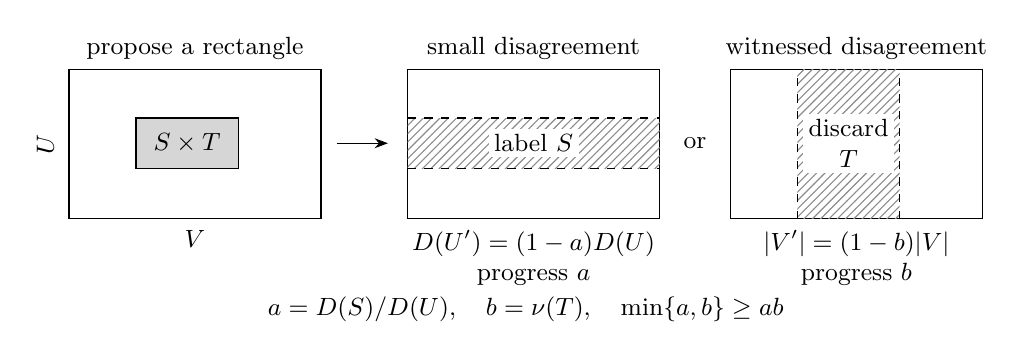
\begin{tikzpicture}[x=1cm,y=1cm,>=Stealth,font=\small]
% Each panel has points on the vertical axis and hypotheses on the horizontal axis.
\begin{scope}
  \draw (0,0) rectangle (3.2,1.9);
  \fill[black!16] (.85,.64) rectangle (2.15,1.28);
  \draw (.85,.64) rectangle (2.15,1.28);
  \node at (1.5,.96) {$S\times T$};
  \node at (1.6,2.17) {propose a rectangle};
  \node[rotate=90] at (-.3,.95) {$U$};
  \node at (1.6,-.25) {$V$};
\end{scope}
\draw[->] (3.4,.96) -- (4.05,.96);
\begin{scope}[xshift=4.3cm]
  \draw (0,0) rectangle (3.2,1.9);
  \fill[pattern=north east lines,pattern color=black!45] (0,.64) rectangle (3.2,1.28);
  \draw[dashed] (0,.64)--(3.2,.64) (0,1.28)--(3.2,1.28);
  \node[fill=white,inner sep=2pt] at (1.6,.96) {label $S$};
  \node at (1.6,2.17) {small disagreement};
  \node[align=center] at (1.6,-.5)
     {$D(U')=(1-a)D(U)$\\progress $a$};
\end{scope}
\node at (7.95,.96) {or};
\begin{scope}[xshift=8.4cm]
  \draw (0,0) rectangle (3.2,1.9);
  \fill[pattern=north east lines,pattern color=black!45] (.85,0) rectangle (2.15,1.9);
  \draw[dashed] (.85,0)--(.85,1.9) (2.15,0)--(2.15,1.9);
  \node[fill=white,inner sep=2pt,align=center] at (1.5,.96) {discard\\$T$};
  \node at (1.6,2.17) {witnessed disagreement};
  \node[align=center] at (1.6,-.5)
     {$|V'|=(1-b)|V|$\\progress $b$};
\end{scope}
\node at (5.8,-1.15) {$a= D(S)/D(U),\quad b=\nu(T),\quad\min\{a,b\}\ge ab$};
\end{tikzpicture}
\caption{An accepted proposal either removes a fraction $a$ of the remaining point mass or a fraction $b$ of the surviving hypotheses. The shaded band marks what is removed. Both updates have progress at least $ab$, the quantity controlled by the pointwise rectangle mixture.}
\label{fig:progress}
\end{figure}


\paragraph{Why it stops.}
Put $a=s/u$ and $b=\nu(T)$. With the tolerance chosen in Appendix~\ref{app:rectangle}, acceptance implies $a\ge r/4$, while every proposal with $a\ge3r/4$ is accepted. A labelling step makes at most $3\tau$ error. An elimination never removes the target.

Assign progress $G=a$ to labelling, $G=b$ to elimination, and $G=0$ to rejection. Either accepted update satisfies $G\ge ab$. Pointwise coverage gives $\E[ab\mid\text{history}]\ge r$, so rejection loses at most $3r/4$ and
\begin{equation}
 \E[G\mid\text{history}]\ge r/4.
 \label{eq:drift}
\end{equation}
The cumulative elimination progress is at most $\ln K$; the cumulative labelling progress is at most $\ln(8/\eps)+1$. An exponential potential therefore bounds the probability of exhausting the round budget. The number of labelling steps is $O(\rho\log(1/\eps))$, explaining the tolerance in \eqref{eq:rectanglebound}. The proof in Appendix~\ref{app:rectangle} treats every allowable oracle answer.

\section{Incidence signs and representation dimension}\label{sec:incidence}
At scale $N$, the point set $X$ and line index set $\Lc$ are both $[N]\times[2N^2]$. A point is $p=(x,y)$ and a line is $\ell=(a,b)$, representing $y=ax+b$. Let
\begin{equation}
 F_{\ell,p}=-1\ \Longleftrightarrow\ y=ax+b.
 \label{eq:grid}
\end{equation}
An incidence flip $A$ changes any subset of these negative entries to $+1$ and leaves every other entry positive. Its row class is $\Hc_A$, and $K=Q=2N^3$. A random flip chooses each incidence sign independently and fairly.

The line $\ell=(1,1)$ is a running example. Its template points are $(1,2),\ldots,(N,N+1)$. Their labels in its row can be chosen arbitrarily; the row remains positive elsewhere. A different line shares at most one of these points, and the two rows' signs at that point are separate random bits.

\begin{figure}[t]
\centering
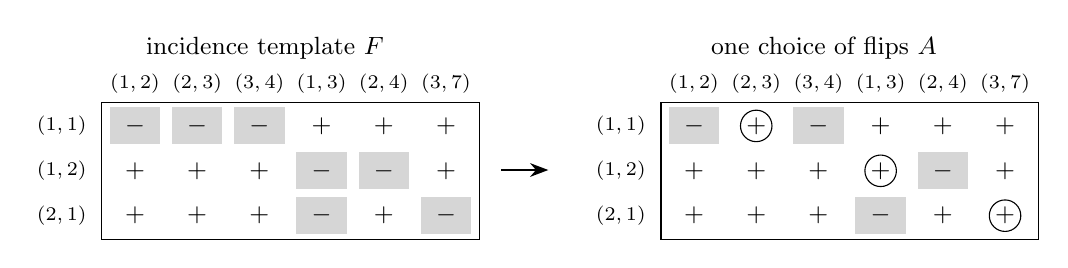
\begin{tikzpicture}[x=1cm,y=1cm,font=\small,>=Stealth]
\begin{scope}[xshift=0cm]
\node at (2.75,2.65) {incidence template $F$};
\node[font=\scriptsize] at (1.1,2.2) {$(1,2)$};
\node[font=\scriptsize] at (1.8900000000000001,2.2) {$(2,3)$};
\node[font=\scriptsize] at (2.68,2.2) {$(3,4)$};
\node[font=\scriptsize] at (3.47,2.2) {$(1,3)$};
\node[font=\scriptsize] at (4.26,2.2) {$(2,4)$};
\node[font=\scriptsize] at (5.050000000000001,2.2) {$(3,7)$};
\node[anchor=east,font=\scriptsize] at (.61,1.66) {$(1,1)$};
\fill[black!16] (0.780,1.425) rectangle (1.420,1.895);
\node at (1.100,1.660) {$-$};
\fill[black!16] (1.570,1.425) rectangle (2.210,1.895);
\node at (1.890,1.660) {$-$};
\fill[black!16] (2.360,1.425) rectangle (3.000,1.895);
\node at (2.680,1.660) {$-$};
\node at (3.470,1.660) {$+$};
\node at (4.260,1.660) {$+$};
\node at (5.050,1.660) {$+$};
\node[anchor=east,font=\scriptsize] at (.61,1.0899999999999999) {$(1,2)$};
\node at (1.100,1.090) {$+$};
\node at (1.890,1.090) {$+$};
\node at (2.680,1.090) {$+$};
\fill[black!16] (3.150,0.855) rectangle (3.790,1.325);
\node at (3.470,1.090) {$-$};
\fill[black!16] (3.940,0.855) rectangle (4.580,1.325);
\node at (4.260,1.090) {$-$};
\node at (5.050,1.090) {$+$};
\node[anchor=east,font=\scriptsize] at (.61,0.52) {$(2,1)$};
\node at (1.100,0.520) {$+$};
\node at (1.890,0.520) {$+$};
\node at (2.680,0.520) {$+$};
\fill[black!16] (3.150,0.285) rectangle (3.790,0.755);
\node at (3.470,0.520) {$-$};
\node at (4.260,0.520) {$+$};
\fill[black!16] (4.730,0.285) rectangle (5.370,0.755);
\node at (5.050,0.520) {$-$};
\draw (.68,.215) rectangle (5.48,1.96);
\end{scope}
\begin{scope}[xshift=7.1cm]
\node at (2.75,2.65) {one choice of flips $A$};
\node[font=\scriptsize] at (1.1,2.2) {$(1,2)$};
\node[font=\scriptsize] at (1.8900000000000001,2.2) {$(2,3)$};
\node[font=\scriptsize] at (2.68,2.2) {$(3,4)$};
\node[font=\scriptsize] at (3.47,2.2) {$(1,3)$};
\node[font=\scriptsize] at (4.26,2.2) {$(2,4)$};
\node[font=\scriptsize] at (5.050000000000001,2.2) {$(3,7)$};
\node[anchor=east,font=\scriptsize] at (.61,1.66) {$(1,1)$};
\fill[black!16] (0.780,1.425) rectangle (1.420,1.895);
\node at (1.100,1.660) {$-$};
\node at (1.890,1.660) {$+$};
\draw (1.890,1.660) circle (.20);
\fill[black!16] (2.360,1.425) rectangle (3.000,1.895);
\node at (2.680,1.660) {$-$};
\node at (3.470,1.660) {$+$};
\node at (4.260,1.660) {$+$};
\node at (5.050,1.660) {$+$};
\node[anchor=east,font=\scriptsize] at (.61,1.0899999999999999) {$(1,2)$};
\node at (1.100,1.090) {$+$};
\node at (1.890,1.090) {$+$};
\node at (2.680,1.090) {$+$};
\node at (3.470,1.090) {$+$};
\draw (3.470,1.090) circle (.20);
\fill[black!16] (3.940,0.855) rectangle (4.580,1.325);
\node at (4.260,1.090) {$-$};
\node at (5.050,1.090) {$+$};
\node[anchor=east,font=\scriptsize] at (.61,0.52) {$(2,1)$};
\node at (1.100,0.520) {$+$};
\node at (1.890,0.520) {$+$};
\node at (2.680,0.520) {$+$};
\fill[black!16] (3.150,0.285) rectangle (3.790,0.755);
\node at (3.470,0.520) {$-$};
\node at (4.260,0.520) {$+$};
\node at (5.050,0.520) {$+$};
\draw (5.050,0.520) circle (.20);
\draw (.68,.215) rectangle (5.48,1.96);
\end{scope}
\draw[->,thick] (5.75,1.1)--(6.35,1.1);
\end{tikzpicture}
\caption{Three lines and six points from the scale-$3$ table. Rows index lines and columns index points. Shading marks negative entries; circles mark incidences flipped to positive. At the shared point $(1,3)$, the signs for lines $(1,2)$ and $(2,1)$ can differ. No two distinct lines share two incidence columns, so a negative rectangle must have a singleton side.}
\label{fig:incidence}
\end{figure}


\begin{proposition}[Geometry and an upper representation]\label{prop:geometry}
Every incidence flip satisfies
\begin{equation}
 \VC(\Hc_A)\le2,\qquad \rect(\Hc_A)\ge2^{-15},\qquad \dc(\Hc_A)\le N+3.
 \label{eq:geometry}
\end{equation}
The template has sign-rank at most six and has exactly
\begin{equation}
 I=2N^4-\bigl(N(N+1)/2\bigr)^2\ge N^4
 \label{eq:incidencecount}
\end{equation}
incidences.
\end{proposition}

\paragraph{Why the geometry survives.}
The score $(ax+b-y)^2-1/2$ gives a six-dimensional strict representation of $F$. The homogeneous-rectangle theorem of \citet{APP05}, in the formulation of \citet[Theorem~1.9]{HHPTZ22}, gives a large monochromatic rectangle under every product distribution. Positive rectangles survive every flip. A nonempty negative rectangle has a singleton side, because distinct lines meet at most once; splitting its other side by the new signs retains at least half its mass. This proves the rectangle bound. The same one-intersection property forbids shattering three points.

A representation needs to store only the labels along each line. Let $q_\ell(t)$ be its label at $(t,at+b)$, taking $+1$ when that point is outside the domain. Then
\begin{equation}
 q_\ell(x)+2(y-ax-b)^2
 \label{eq:representation-score}
\end{equation}
has the desired sign. It is linear in the $N+3$ features $\one_{\{x=t\}}$, $t\in[N]$, and $y,xy,y^2$. On the running line $y=x+1$, its score is exactly the chosen incidence sign. At every other grid point the squared residual is at least one, so the score is positive. Appendix~\ref{app:geometry} gives the coefficients and the incidence count.

\subsection{Counting on the incidence support}
The lower bound must count the part of the table that actually varies. Off-incidence entries contain no random information.

\begin{lemma}[Restricted sign patterns]\label{lem:mask}
For an integer $d\ge1$, on a specified set $J$ of $s$ entries of a $k\times q$ matrix, the number of strict sign patterns produced by real matrices of rank at most $d$ is at most
\begin{equation}
 \left(\frac{8es}{v}\right)^v,\qquad v=(k+q)d,\quad 1\le v\le s.
 \label{eq:maskcount}
\end{equation}
\end{lemma}

\begin{proof}
Factor the matrix into $k$ row vectors and $q$ column vectors in $\R^d$. Its entries in $J$ are $s$ degree-two polynomials in $v$ variables. Apply the strict-sign form of \citet{Warren68}; this factorization argument is standard in sign-rank counting \citep{AMY16}.
\end{proof}

For $0\le\eta<1/2$, let $\hbin(\eta)=-\eta\log_2\eta-(1-\eta)\log_2(1-\eta)$, with $0\log_2 0=0$, and set
\begin{equation}
 c_\eta=1-\hbin(\eta),\qquad
 s_\eta=\left\lfloor\frac{c_\eta^2 I}{32(K+Q)}\right\rfloor.
 \label{eq:seta}
\end{equation}
Lemma~\ref{lem:mask} counts at most $2^{c_\eta I/2}$ patterns in rank $s_\eta$; a Hamming ball of radius $\eta I$ contains at most $2^{\hbin(\eta)I}$ patterns. Their union covers at most a $2^{-c_\eta I/2}$ fraction of the random signs.

\begin{lemma}[Probabilistic reductions]\label{lem:prob-reduction}
If $\dc_\eta(\Hc_A)=d$, a strict matrix of rank at most $d+1$ makes at most $\eta I$ errors on the incidences. For every finite class,
\begin{equation}
 \dc_{1/4}(\Hc)\le\edc(\Hc)+1.
 \label{eq:exact-to-average}
\end{equation}
\end{lemma}

\paragraph{Why randomization does not evade the count.}
For each nonempty line support $J_\ell$, use the uniform marginal on $J_\ell$ and weight the row by $|J_\ell|/I$. The expected total incidence error is at most $\eta I$, so one embedding attains that bound. Make its predictions strict with the constant feature. For \eqref{eq:exact-to-average}, the constant feature provides a predictor of error at most $1/2$ whenever exact representation fails; failure has probability at most $1/2$. Appendix~\ref{app:counting} gives the full reductions.

\begin{theorem}[Dimension probabilities]\label{thm:dimensions}
A random incidence flip satisfies
\begin{align}
 \Pr[\dc(\Hc_A)\le s_0]&\le2^{-I/2},\label{eq:ordinaryprob}\\
 \Pr[\dc_\eta(\Hc_A)<s_\eta]&\le2^{-c_\eta I/2},\label{eq:averageprob}\\
 \Pr[\edc(\Hc_A)<s_{1/4}-1]&\le2^{-c_{1/4}I/2}.
 \label{eq:exactprob-bound}
\end{align}
\end{theorem}

Since $I\ge N^4$ and $K+Q=4N^3$, the thresholds are linear in $N$ for each fixed error. Proposition~\ref{prop:geometry} supplies the matching upper bound. Thus approximation and randomization leave the order of dimension unchanged for this family.

\section{Allowing a prior and discarding targets}\label{sec:prior}
A stronger relaxation chooses the feature law for a known target prior and requires it to work only for most targets. This is the average probabilistic dimension of \citet[Definition~3.2]{KM25}. We denote it by $\adc_{\eta,\delta}(\pi)$ and use Boolean threshold loss: it is the least $d$ admitting one law on maps $\phi:X\to\R^d$ with
\begin{equation}
 \Pr_{h\sim\pi}\left[\ \forall D\in\Delta(X),\quad
       \E_\phi\mathcal E_\phi(D,h)\le\eta\ \right]\ge1-\delta.
 \label{eq:adcdef}
\end{equation}
The law may depend on $\pi$. It may not depend on the realized target or on $D$. The good set of targets must work for every marginal.

\begin{theorem}[Dimension after discarding targets]\label{thm:prior}
Let $\Lc_0=[N]\times[N^2]$ be the full-length lines, let $L=|\Lc_0|=N^3$, and let $\pi_N$ be the prior on $\Hc_A$ induced by a uniform line in $\Lc_0$. Fix $0\le\eta<1/2$ and $0\le\delta<1$. Put
\begin{equation}
 g=\ceil{(1-\delta)L},\qquad
 t_{\eta,\delta}=\left\lfloor\frac{c_\eta^2 gN}{32(g+Q)}\right\rfloor.
 \label{eq:prior-threshold}
\end{equation}
Then
\begin{equation}
 \Pr_A[\adc_{\eta,\delta}(\pi_N)<t_{\eta,\delta}]
 \le \binom{L}{g}\,2^{-c_\eta gN/2}.
 \label{eq:prior-prob}
\end{equation}
Consequently $\adc_{\eta,\delta}(\pi_N)=\Theta_{\eta,\delta}(N)$ with probability $1-\exp(-\Omega_{\eta,\delta}(N^4))$.
\end{theorem}

\begin{proofsketch}
Fix $g$ rows. Their $gN$ incidence signs are independent. An embedding that approximates all these rows under every marginal gives, by testing on each row's line, an approximation of rank at most $d+1$ to these signs. Apply Lemma~\ref{lem:mask} with $g$ rows and $Q$ columns, then count nearby patterns. Finally take a union bound over the $\binom{L}{g}$ possible good row sets. Their logarithmic number is only $O(N^3)$; the random signs supply $\Theta(N^4)$ bits. Appendix~\ref{app:prior} proves the statement, including priors with repeated functions.
\end{proofsketch}

Even retaining only $1\%$ of the targets requires dimension linear in $N$. The constant depends on the retained fraction and the approximation error; the order does not.

The next proposition explains how the prior-average notion relates to a worst-target guarantee. It replaces the family of laws chosen separately for all priors by one common law, at a controlled increase in error.

\begin{proposition}[From all priors to all targets]\label{prop:prior-minimax}
For every finite class, $0\le\eta<1/2$, and $0\le\delta<1$, put $\theta=\eta+(1/2-\eta)\delta$. Then
\begin{equation}
 \dc_\theta(\Hc)-1
 \le \sup_{\pi\in\Delta(\Hc)}\adc_{\eta,\delta}(\pi)
 \le \dc_\eta(\Hc).
 \label{eq:prior-minimax}
\end{equation}
\end{proposition}

For the left inequality, append a constant feature. Good targets have expected error at most $\eta$; the remaining targets can use a constant predictor of error at most $1/2$. Hence every mixture of target--marginal pairs admits a feature law of average loss at most $\theta$. Minimax supplies one law for all pairs. The argument reduces feature maps to the finitely many Boolean prediction families they induce, rather than assuming compactness of real-valued maps. Appendix~\ref{app:prior} proves this reduction.

\subsection{Classical SQ dimension and a claimed representation bound}\label{sec:km}
The same construction separates prior-average representation from classical SQ dimension. Define $\sqdim(\Hc,D)$ as the largest number $d$ of distinct hypotheses satisfying $\E_D[h_i h_j]\le1/d$ for $i\ne j$, and put $\sqdim(\Hc)=\max_D\sqdim(\Hc,D)$. This is the one-sided correlation convention of \citet[Definition~3.5]{KM25}. Classical SQ dimension does not characterize distribution-independent strong learning \citep{Feldman17}.

\begin{proposition}[Rectangles bound classical SQ dimension]\label{prop:classical-sq}
For every finite nonempty class,
\begin{equation}
 \sqdim(\Hc)\le 2/\rect(\Hc).
 \label{eq:classical-sq}
\end{equation}
In particular, every incidence flip has $\sqdim(\Hc_A)\le2^{16}$.
\end{proposition}

On a monochromatic rectangle, the sum of $t$ selected hypotheses has squared magnitude $t^2$. The correlation bounds limit its expected square to $t+t(t-1)/d$, giving \eqref{eq:classical-sq}; see Appendix~\ref{app:prior}. Thus classical SQ dimension stays bounded while Theorem~\ref{thm:prior}'s prior-average dimension tends to infinity. No function of classical SQ dimension alone can bound the latter at fixed $\eta<1/2$ and $\delta<1$.

\citet[Theorem~4.1]{KM25} claim $\adc_{\eta,\delta}(\pi)=O(\sqdim(\Hc)^{24.01})$ for small fixed errors. \citet{FKS26} already report that the ``claimed upper bounds do not hold due to a flaw in the proof,'' citing a personal communication from Karchmer and Malach. Theorem~\ref{thm:prior} and Proposition~\ref{prop:classical-sq} give an explicit counterexample to Theorem~4.1 under its stated fixed-feature-law quantifiers, consistent with that report. The lower bound uses Boolean threshold loss and therefore also applies to their literal unthresholded $0$--$1$ loss, which is no smaller.

The proof of their mini-batch SGD theorem, Theorem~3.3, invokes Theorem~4.1. Our counterexample rules out that intermediate implication; it does not disprove the mini-batch SGD conclusion itself. Open Question~1 of \citet{FKS26} is separate. That question specifies an architecture and training procedure rather than formally defining a class of ``benign'' networks.

\section{Query optimality and general dimension bounds}\label{sec:optimality}
The learning upper bound holds for every flip, including the all-positive table, so a query lower bound cannot hold for every member. For random incidence signs, we now show that logarithmically many queries are necessary at fixed tolerance. The learner may know the entire realized table.

\begin{theorem}[Query lower bounds]\label{thm:querylower}
Let $\chi=1-\hbin(3/8)$. Suppose the integer $N\ge2$ satisfies $\chi N\ge6\log_2N$ (equivalently, $N\ge1373$). With probability at least $1-2^{-2N^3}-N^3e^{-N/32}$ over $A$, every randomized learner satisfying \eqref{eq:learnmodel}, for any $0<\eps<1/4$ and $0<\tau<1$, obeys
\begin{equation}
 m\ge\frac{\log_2 N+\log_2\!\bigl(\chi(1-8\eps/3)/8\bigr)}{\log_2\ceil{1/\tau}}.
 \label{eq:lowerimproper}
\end{equation}
If its output must belong to $\Hc_A$, then
\begin{equation}
 m\ge\frac{3\log_2 N+\log_2(1-3\eps)}{\log_2\ceil{1/\tau}}.
 \label{eq:lowerproper}
\end{equation}
The bounds already hold on targets from $\Lc_0$, with the uniform marginal on each target line.
\end{theorem}

\paragraph{Why outputs, not targets, must be counted.}
A fixed predictor fits a random row on its $N$ incidences with probability exponentially small in $N$. Counting all predictors shows that none fits more than $O(N^2)$ of the $N^3$ full-line instances. Quantizing the replies gives at most $\ceil{1/\tau}^m$ outputs for each fixed learner seed. Averaging over seeds proves \eqref{eq:lowerimproper}. A proper output fits at most one line instance, giving \eqref{eq:lowerproper}. An improper output can fit every line of one slope simultaneously, so the stronger proper bound cannot be obtained by counting target labels alone. Appendix~\ref{app:query} supplies both arguments.

The response tree also gives a converse bound on representation dimension. Its leaf predictors can serve as features, regardless of how the learner computes them. The next proposition extends this observation to all three dimension notions.

\begin{proposition}[Transcript representations]\label{prop:transcript}
Suppose a randomized depth-$m$ learner achieves expected error $\eps<1/2$ at tolerance $0<\tau<1$. Put $B_\tau=\ceil{1/\tau}$ and $\gamma=1-2\eps$. Then
\begin{align}
 \dc_\eps(\Hc)&\le B_\tau^m,\label{eq:transcript}\\
 \edc(\Hc)&\le B_\tau^m\ceil{2\gamma^{-2}\ln(2Q)},\label{eq:transcript-exactprob}\\
 \dc(\Hc)&\le B_\tau^m\ceil{2\gamma^{-2}\ln(2KQ)}.\label{eq:transcript-exact}
\end{align}
For a deterministic learner, $\dc(\Hc)\le B_\tau^m$.
\end{proposition}

For each learner seed, use all $B_\tau^m$ leaf outputs as coordinates. The rounded oracle selects one of them, proving \eqref{eq:transcript}. For exact representation, minimax converts the guarantee under every marginal into row-specific convex combinations with positive expected signed score at every point. Concatenating independent leaf maps and applying concentration proves \eqref{eq:transcript-exactprob}--\eqref{eq:transcript-exact}. Appendix~\ref{app:query} gives the full argument.

At fixed tolerance, the incidence separation attains the exponential order in $m$ allowed by these bounds. We do not claim that the logarithmic overhead for exact representations is necessary.

\begin{figure}[t]
\centering
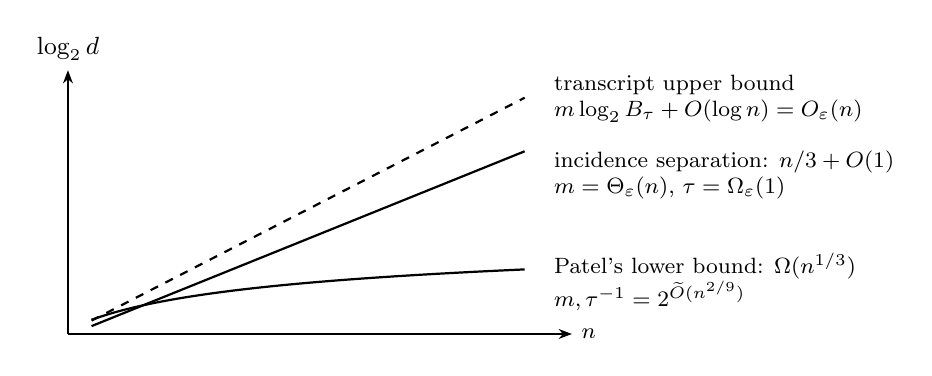
\begin{tikzpicture}[x=1cm,y=1cm,>=Stealth,font=\small]
 \draw[->] (0,0)--(6.4,0) node[right,font=\footnotesize] {$n$};
 \draw[->] (0,0)--(0,3.35) node[above] {$\log_2 d$};
 \draw[dashed,thick] (.3,.17)--(5.8,3.0);
 \draw[thick] (.3,.1)--(5.8,2.32);
 \draw[thick] (.3,.18) .. controls (1.2,.51) and (2.9,.69) .. (5.8,.82);
 \node[anchor=west,align=left,font=\footnotesize] at (6.05,2.99)
   {transcript upper bound\\$m\log_2 B_\tau+O(\log n)=O_\eps(n)$};
 \node[anchor=west,align=left,font=\footnotesize] at (6.05,2.02)
   {incidence separation: $n/3+O(1)$\\$m=\Theta_\eps(n)$, $\tau=\Omega_\eps(1)$};
 \node[anchor=west,align=left,font=\footnotesize] at (6.05,.66)
   {Patel's lower bound: $\Omega(n^{1/3})$\\$m,\tau^{-1}=2^{\widetilde O(n^{2/9})}$};
\end{tikzpicture}
\caption{Growth orders of log dimension at fixed learning and representation errors; constants are suppressed. The incidence bound holds for all three dimension notions and meets the exponential order of the transcript bound at its own query resources. The dashed line uses $K=Q=2^n$, $m=\Theta_\eps(n)$, and fixed tolerance; it is not the upper bound at Patel's resources. Patel's curve denotes an ordinary-dimension lower bound, not an upper bound on his class.}
\label{fig:parameters}
\end{figure}


\section{Computational implementations}\label{sec:computation}
The statistical separation charges queries, not the size of the class description. Its computational content depends on whether the learner receives the full table or a short entry evaluator.

\begin{theorem}[Table and succinct implementations]\label{thm:table}
For every $0<\eps<1/4$, each incidence flip has the deterministic proper table-polynomial learner in \eqref{eq:mainlearn}. If its entries can instead be evaluated in time $E(n)$, it has a deterministic improper learner using $O(n^2)$ queries of tolerance $\eps/8192$, with computation polynomial in $(n,1/\eps,E(n))$ and an efficiently evaluable output.
\end{theorem}

The table algorithm derives a constant-size catalog of geometric rectangles from the six-dimensional template, then chooses useful rectangles deterministically. At the first negative labelling step, the one-intersection property either identifies a good row or locates a negative point. The remaining row supports away from that point are disjoint, which permits proper completion. Appendix~\ref{app:proper} gives a finite-bit implementation.

The succinct algorithm uses the order along a line. At a trial slope $a$, the residual $y-ax$ increases with $x$ if $a$ is too small and decreases if it is too large. Noisy medians and one intersection-mass query distinguish these cases. A heavy atom identifies either the whole line or one negative point. This yields $O(\log N)$ stages with $O(\log N)$ queries each. Appendix~\ref{app:median} proves the result and a proper variant under a condition satisfied by almost every random table.

A succinct separation follows under a cryptographic assumption. Under the direct subexponential pseudorandom-function assumption stated in Appendix~\ref{app:prf}, for every prescribed integer $c\ge1$ there are polynomial-length keys such that almost every key defines a class with all three dimensions at least $n^c$ and a key-known randomized proper polynomial-time learner using $O_\eps(n^2)$ queries at fixed tolerance. Every key has the deterministic improper learner. The key-length exponent depends on $c$; this does not give an unconditional succinct construction, or an exponential gap for one polynomial-time family.

\section{Discussion}\label{sec:open}
The separation is sharp in dimension for the incidence construction and in query order at fixed tolerance. Its exponential gap still relies on an unstructured table: the counting argument does not choose a high-dimension flip with an unconditional polynomial-time evaluator. The conditional succinct families give each prescribed polynomial dimension separately, not this exponential gap. The full dependence on a varying tolerance remains undetermined. None of these SQ results resolves the separate gradient-descent question.

\ifreview\else
\acks{GPT-6 Astra and GPT-6 Astra Pro (OpenAI) assisted with mathematical development, source comparison, code, and writing. Claude (Anthropic) assisted with the Lean formalization. The author is responsible for the results and presentation.}
\fi
\paragraph{Reproducibility.}
The source includes complete proofs, build instructions, and finite arithmetic checks. The Lean development checks 213 supporting theorems for incidence geometry, the classical-SQ bound, noisy medians, conditional counting and query bounds, and the rectangle learner's proof steps. Its coverage table records the external hypotheses and the parts not yet formalized; no whole-paper formal verification is claimed.
\label{main-end}

\bibliography{references}
\clearpage
\appendix
\section{Proof of the rectangle learning theorem}\label{app:rectangle}
We prove Theorem~\ref{thm:rectangle}. The two progress measures have bounded total size, so it suffices to force a positive conditional drift while keeping each labelling error small. Fix
\begin{align}
 r&=1/\rho,\qquad P=1+\ceil{4r^{-1}\ln(8/\eps)},\qquad
 \tau=\frac{\eps}{24P},\label{eq:rectparams1}\\
 B&=\ln K+\ln(8/\eps)+1,\qquad
 R=\ceil{8r^{-1}(B+\ln(2/\eps))}.\label{eq:rectparams2}
\end{align}
Run the algorithm in Section~\ref{sec:rectangle} for at most $R$ rounds, using $\tau$ for every query. An empty residual terminates immediately. At any termination extend the assigned predictor by $+1$. The claimed worst-case budget is $3R+1$.

The only randomness in the argument is the choice of rectangle. All inequalities concerning answers hold for every valid response, including either endpoint of its allowed interval.

\subsection{The minimax distribution}
For completeness, the finite minimax statement used in Lemma~\ref{lem:mixture} can be written as a linear program. Enumerate the monochromatic rectangles of $U\times V$ as $\Rc$, and put
\[
 z_R(x)=\one_{S_R}(x)\nu(T_R)\quad(R\in\Rc,\ x\in U).
\]
The required distribution is a feasible solution of
\begin{equation}
 \lambda_R\ge0,\qquad \sum_{R\in\Rc}\lambda_R=1,
 \qquad \sum_{R\in\Rc}\lambda_R z_R(x)\ge r\quad(x\in U).
\label{eq:mixture-lp}
\end{equation}
If the convex hull of the vectors $z_R$ did not intersect $[r,\infty)^U$, a separating hyperplane could be chosen with nonnegative normal vector: the latter set is closed under adding any nonnegative vector. Normalize this normal vector to a probability distribution $\mu$ on $U$. Separation would give $\max_R\mu(S_R)\nu(T_R)<r$, contradicting the rectangle hypothesis on the restriction. This proves feasibility.

In the application, $\nu$ is uniform on the surviving rows. When $r$ is rational, \eqref{eq:mixture-lp} has rational coefficients and admits a rational feasible point. For a supplied real lower bound one may use a positive rational bound within a constant factor. This observation concerns constructibility; the number of variables in the general program can still be exponential.

\subsection{Valid answers and the two updates}
Fix $D$, a target $h^*\in\Hc$, and a valid adaptive oracle. Condition on any nonstopping history, including the answer to the current residual-mass query. Let
\[
 u=D(U),\quad s=D(S),\quad
 w=D(S\cap\{h^*\ne c\}),\quad
 a=s/u,\quad b=|T|/|V|.
\]
The parameter choice gives
\begin{equation}
 \tau\le\eps/8,\qquad \tau\le r\eps/64.
\label{eq:tau-small}
\end{equation}
Indeed, $P\ge4r^{-1}\ln(8/\eps)$ and $\ln(8/\eps)>\ln32$. Since the algorithm did not stop,
\begin{equation}
 u>\eps/4-\tau\ge\eps/8,
 \qquad \tau/u\le r/8.
\label{eq:active-mass}
\end{equation}
If the proposal is accepted, then $\hat s\ge r\hat u/2$, and therefore
\[
 s\ge ru/2-(1+r/2)\tau.
\]
Using $r\le1$ and \eqref{eq:active-mass}, we obtain
\begin{equation}
 a\ge r/2-(1+r/2)r/8\ge5r/16\ge r/4.
\label{eq:accepted-mass}
\end{equation}
Conversely, if $a\ge3r/4$, then even the least favorable answers obey
\[
 \hat s-r\hat u/2
 \ge (a-r/2)u-(1+r/2)\tau
 \ge ru/4-3ru/16=ru/16>0.
\]
Every such proposal is accepted.

When $\hat w\le2\tau$, the labelling step incurs error $w\le3\tau$. When $\hat w>2\tau$, the target cannot lie in $T$: monochromaticity would then give $w=0$ and $\hat w\le\tau$. Thus every elimination retains the target and leaves $V$ nonempty. These conclusions hold for both endpoints of every allowed answer interval.

\subsection{Deterministic bounds on total progress}
There are at most $P$ labelling steps. Before the $j$th such step, \eqref{eq:accepted-mass} implies
\[
 \eps/8\le u\le(1-r/4)^{j-1}\le e^{-(j-1)r/4}.
\]
Consequently $j\le1+4r^{-1}\ln(8/\eps)\le P$. The labelled sets are disjoint, so their total error is at most
\begin{equation}
 3P\tau=\eps/8.
\label{eq:peel-error}
\end{equation}
At an ordinary stop, the residual mass is at most $\eps/4+\tau$. An empty residual contributes no error. In either case the final loss is bounded by
\begin{equation}
 \eps/8+\eps/4+\tau\le\eps/2.
\label{eq:normal-loss}
\end{equation}

For an elimination with row fraction $b$, the uniform target weight is multiplied by $1/(1-b)$. Since it starts at $1/K$ and cannot exceed one,
\begin{equation}
 \sum_{\text{eliminations}}b
 \le\sum_{\text{eliminations}}-\ln(1-b)
 \le\ln K.
\label{eq:elim-charge}
\end{equation}
Here $b<1$, because the target is retained.

For the labelling steps, exclude the last one. The residual masses telescope through all preceding steps, and the mass just before the last is at least $\eps/8$. Hence
\[
 \sum_{\text{labelling steps except the last}}a
 \le\sum_{\text{same steps}}-\ln(1-a)
 \le\ln(8/\eps).
\]
Adding the last charge, which is at most one, gives
\begin{equation}
 \sum_{\text{labelling steps}}a\le\ln(8/\eps)+1.
\label{eq:peel-charge}
\end{equation}
If a step removes all remaining points, it is necessarily the last step, so no logarithm of zero occurs. With no labelling steps the inequality is immediate.

Define $G_t=a$ on a labelling step, $G_t=b$ on an elimination, and $G_t=0$ on a rejected proposal. Equations~\eqref{eq:elim-charge} and \eqref{eq:peel-charge} show that, before normal termination,
\begin{equation}
 \sum_t G_t\le B.
\label{eq:total-charge}
\end{equation}
The bound holds for every realized history.

\subsection{Expected progress and the query budget}
Integrating \eqref{eq:pointwise} against $D$ conditioned on $U$ gives
\[
 \E[ab\mid\text{current history}]\ge r.
\]
On acceptance either update has $G_t\ge ab$, since $a,b\le1$. Rejection is possible only when $a<3r/4$, and its contribution to $\E[ab]$ is at most $(3r/4)\E b\le3r/4$. Therefore
\begin{equation}
 \E[G_t\mid\text{current history}]\ge r/4.
\label{eq:drift-app}
\end{equation}
The oracle may select any allowed mismatch answer after seeing the rectangle. This cannot invalidate the inequality: both possible accepted updates dominate $ab$.

Extend $G_t$ to equal one after normal termination. Since $0\le G_t\le1$, convexity gives
\[
 e^{-G_t}\le1-(1-e^{-1})G_t.
\]
Conditioning first on the current residual-mass answer when necessary, \eqref{eq:drift-app} yields
\[
 \E[e^{-G_t}\mid\text{past}]
 \le1-r/8\le e^{-r/8}.
\]
Iterating conditional expectation gives
\begin{equation}
 \E\exp\!\left(-\sum_{t=1}^{R}G_t\right)\le e^{-rR/8}.
\label{eq:exponential-potential}
\end{equation}
On an execution that exhausts the budget without a normal stop, \eqref{eq:total-charge} gives $\sum_{t=1}^R G_t\le B$. Markov's inequality and \eqref{eq:exponential-potential} therefore imply
\[
 \Pr[\text{budget exhaustion}]
 \le e^{B-rR/8}\le\eps/2.
\]
Combining this with \eqref{eq:normal-loss} and the trivial loss bound one proves expected loss at most $\eps$. There are at most three queries per round, so $3R+1$ is a valid worst-case bound. Substituting the definitions of $P$ and $R$ proves \eqref{eq:rectanglebound}.

A randomized oracle is handled by conditioning on its past randomness. Nothing in the proof grants it access to the learner's future coins. Conversely, the learner does not rely on any stochastic model for the oracle's errors. This completes the proof of Theorem~\ref{thm:rectangle}.

\section{Geometry of the separating family}
\label{app:geometry}
The construction uses geometry only to protect rectangles and uses indicator features to memorize signs along a line. We first check the geometric assertions, then exhibit the common feature map proving Proposition~\ref{prop:geometry}.

Two different lines in $\Lc$ share at most one point. Hence their negative supports in any monotone flip share at most one point. In particular, the table contains no all-negative $2\times2$ submatrix. If three points were shattered, the row negative on all three and the row negative on exactly two of them would share two negative points. Thus the VC dimension is at most two.

The template is strictly represented by the polynomial
\[
 (ax+b-y)^2-\tfrac12
 =a^2x^2-2axy+y^2+2abx-2by+b^2-\tfrac12.
\]
All coordinates are integers. The expression is negative exactly at an incidence and positive otherwise. Its six displayed point monomials give $\sr(F)\le6$.

We use the following homogeneous-rectangle theorem: a sign matrix of sign-rank at most $d$ has a monochromatic rectangle occupying at least a $2^{-d-1}$ fraction of its rows and a $2^{-d-1}$ fraction of its columns \citep{APP05}. It also holds under arbitrary product weights, with product mass at least $2^{-2d-2}$. For rational weights, duplicate each row and column according to its weight and apply the unweighted theorem. Project the resulting rectangle back to the original row and column sets. The projected mass is at least the selected mass in the duplicated matrix. For real weights, approximate by rational distributions. There are finitely many rectangles, so the maximum of their product masses is continuous. Passing to the limit proves the weighted assertion. This is the weighted form recorded by \citet[Theorem 1.9]{HHPTZ22}.

For the rank-six template, every product distribution therefore has a monochromatic rectangle of mass at least $2^{-14}$. A positive rectangle remains positive after flipping. A nonempty negative rectangle has a singleton side, because there is no negative $2\times2$. Partition the other side according to its labels in $A$. The heavier part retains at least half the rectangle's product mass and is monochromatic in $A$. Thus $\rect(\Hc_A)\ge2^{-15}$.

To count incidences, fix $a,x\in[N]$. A positive intercept $b$ gives a grid incidence precisely when $b\le2N^2-ax$. Since $ax\le N^2$, this quantity is positive. Summing gives
\[
 I=\sum_{a=1}^{N}\sum_{x=1}^{N}(2N^2-ax)
 =2N^4-\left(\sum_{a=1}^{N}a\right)^2
 =2N^4-\left(\frac{N(N+1)}2\right)^2.
\]
The inequality $I\ge N^4$ follows from $(N+1)^2\le4N^2$. Each incidence corresponds to a different matrix entry, so all $I$ signs can be chosen independently. Row $(1,2N^2)$ has no incidences and remains the all-positive hypothesis.

Finally, use the $N+3$ features described after \eqref{eq:representation-score}. Give the feature $\one_{x=t}$ weight
\[
 q_\ell(t)+2(at+b)^2,
\]
and give $y,xy,y^2$ weights $-4b,-4a,2$, respectively. The resulting score is exactly \eqref{eq:representation-score}. On incidences it equals $q_\ell(x)=A_{\ell,(x,y)}$. Off incidences, the squared integer residual is at least one, and the score is at least $-1+2=1$. This is a strict common representation. Choosing it deterministically also bounds both probabilistic dimensions by $N+3$.

\section{Dimension lower bounds on the incidence support}
\label{app:counting}
\subsection{Restricted sign-pattern counting}
The proof counts the random signs rather than their fixed completion. We use the following version for arbitrary masks, including the row subsets needed in Appendix~\ref{app:prior}.
\begin{lemma}[Approximation on a random mask]\label{lem:mask-approx}
Let $J$ contain $I>0$ entries in a $K\times Q$ matrix, with independent fair signs on $J$. For $0\le\eta<1/2$, set
\[
 s_\eta=\left\lfloor\frac{c_\eta^2 I}{32(K+Q)}\right\rfloor.
\]
The probability that some real matrix of rank at most $s_\eta$, strict on $J$, disagrees with at most $\eta I$ signs is at most $2^{-c_\eta I/2}$.
\end{lemma}
We prove Lemmas~\ref{lem:mask} and~\ref{lem:mask-approx}. The form of Warren's theorem we use is the following: $s$ polynomials of degree at most $k$ in $v$ real variables, with $s\ge v$, attain at most $(4eks/v)^v$ strict sign patterns \citep{Warren68}. For a presentation in the sign-rank setting, see \citet{AMY16}.

A rank-at-most-$d$ real $K$ by $Q$ matrix has a factorization $UV$, with $U\in\R^{K\times d}$ and $V\in\R^{d\times Q}$. Its entry at $(i,j)$ is
\[
 p_{ij}(U,V)=\sum_{t=1}^{d}U_{it}V_{tj}.
\]
Restrict to $(i,j)\in J$. These are $I$ polynomials of degree two in $v=(K+Q)d$ variables. It is irrelevant whether an unexamined entry vanishes. Warren's theorem gives
\[
 \#\{\text{strict patterns on }J\}
 \le (8eI/v)^v,
\]
which proves \eqref{eq:maskcount}. In particular, this step does not count completions of the partial sign pattern, and it does not charge for fixed off-support entries.

The number of sign vectors within Hamming distance $\eta I$ of a fixed vector is at most $2^{\hbin(\eta)I}$. For $0<\eta<1/2$, expand
\[
 1=(\eta+(1-\eta))^I.
\]
Each term of weight $j\le\eta I$ has factor $\eta^j(1-\eta)^{I-j}$ at least $\eta^{\eta I}(1-\eta)^{(1-\eta)I}$, because $\eta/(1-\eta)<1$. The bound follows by dividing by this factor. For $\eta=0$ the ball consists of one vector.

Let $c=c_\eta\in(0,1]$ and suppose $s_\eta\ge1$. With $d=s_\eta$ and $x=v/I$, the threshold in \eqref{eq:seta} gives $x\le c^2/32$. The function $x\log_2(8e/x)$ is increasing for $0<x\le1$. Therefore
\begin{align*}
 \frac1I\log_2\#\{\text{rank-}d\text{ patterns on }J\}
 &\le \frac{c^2}{32}\log_2\left(\frac{256e}{c^2}\right)\\
 &\le c/2.
\end{align*}
For the last inequality, put $f(c)=c\log_2(256e/c^2)$. Its derivative is
\[
 f'(c)=\log_2(256e/c^2)-2/\ln2>0\qquad(0<c\le1).
\]
Hence $f(c)\le f(1)=\log_2(256e)<16$. Also $v\le I$, as required by Warren's theorem.

There are $2^I$ equally likely random sign vectors. A union bound over the rank-$d$ patterns and their Hamming balls now gives
\[
 \Pr[\text{a rank-}d\text{ pattern has at most }\eta I\text{ errors}]
 \le 2^{cI/2+\hbin(\eta)I-I}
 =2^{-cI/2}.
\]
If $s_\eta=0$, no rank-zero matrix is strict on a nonempty set of entries. The event is empty. This proves every case of Lemma~\ref{lem:mask-approx}.

\subsection{A single embedding for the incidence test}
We prove the first assertion of Lemma~\ref{lem:prob-reduction}. Let $J_\ell$ be the template incidence support of row $\ell$, and let $k_\ell=|J_\ell|$. Then $\sum_\ell k_\ell=I$. Suppose a law on $d$-dimensional feature maps witnesses $\dc_\eta(\Hc_A)=d$. For each row with $k_\ell>0$, apply \eqref{eq:avgprob} to the uniform distribution on $J_\ell$:
\[
 \E_\phi\min_w\frac1{k_\ell}
 \sum_{z\in J_\ell}\one\{\sgn\ip{w}{\phi(z)}\ne A_{\ell,z}\}
 \le\eta.
\]
Multiply by $k_\ell/I$ and sum over the nonempty rows. Empty rows receive weight zero, so no probability distribution on an empty set is used. Linearity of expectation gives
\begin{equation}
 \E_\phi\sum_{\ell:k_\ell>0}\frac{k_\ell}{I}
 \min_w\err_{\Unif(J_\ell),h_\ell}(\sgn\ip{w}{\phi})
 \le\eta.
\label{eq:weighted-incidence}
\end{equation}
The quantity inside the expectation is a multiple of $1/I$. For each fixed embedding, the rowwise minima are attained by Boolean patterns. Thus some single embedding makes the quantity at most $\eta$.

For that embedding, choose one minimizing vector for each nonempty row, and choose any vector for the remaining rows. This produces a real score matrix of rank at most $d$ whose thresholded predictions make at most $\eta I$ incidence mistakes. Strictify all its Boolean signs as in Remark~\ref{rem:ties}. The resulting strict score matrix has rank at most $d+1$, without changing any of the predictions. If $d<s_\eta$, then $d+1\le s_\eta$, which gives the event implication used in Theorem~\ref{thm:dimensions}.

This argument uses one embedding for every row. It does not choose a different feature map for each target distribution. The use of different row distributions is legitimate because the law on embeddings in \eqref{eq:avgprob} is independent of both the marginal and the target.

\subsection{Exact probabilistic representations}
We prove \eqref{eq:exact-to-average} directly. Let a law on maps $\phi:X\to\R^d$ witness exact probabilistic dimension $d$. Append a constant coordinate to obtain $\widetilde\phi(z)=(\phi(z),1)$. For any fixed $D,h$, on the exact-success event the old weights, with a zero final coordinate, give zero error. On every other outcome, one of the two constant predictors has error at most $1/2$. Both constants are linear predictors in $\widetilde\phi$. Consequently
\[
 \E_{\widetilde\phi}\min_w
 \err_{D,h}(\sgn\ip{w}{\widetilde\phi})
 \le \tfrac12\Pr[\text{exact representation fails}]
 \le\tfrac14.
\]
The augmented embedding law still does not depend on $D,h$. This proves $\dc_{1/4}(\Hc)\le d+1$. More generally, exact representation with probability at least $p>0$ gives expected error at most $(1-p)/2$ after one constant coordinate. No amplification or union bound over hypotheses is needed.

\subsection{The dimension theorem and the negative answer}
For ordinary dimension, a strict rank-at-most-$s_0$ representation of the whole table restricts to such a pattern on the incidence set. Apply Lemma~\ref{lem:mask-approx} at $\eta=0$ to obtain \eqref{eq:ordinaryprob}.

For expected-error dimension, the first part of Lemma~\ref{lem:prob-reduction} and the same counting lemma give \eqref{eq:averageprob}. For exact probabilistic dimension, the event
\[
 \edc(\Hc_A)<s_{1/4}-1
\]
implies $\dc_{1/4}(\Hc_A)<s_{1/4}$ by \eqref{eq:exact-to-average}. Equation~\eqref{eq:averageprob} with $\eta=1/4$ proves \eqref{eq:exactprob-bound}. This proves Theorem~\ref{thm:dimensions}.

Since $I\ge N^4$ and $K+Q=4N^3$, the thresholds satisfy
\[
 s_0\ge N/128-1,\qquad
 s_\eta\ge c_\eta^2N/128-1.
\]
Intersect the three dimension events. Their failure probabilities sum to at most
\[
 2^{-I/2}+2^{-c_\eta I/2}+2^{-c_{1/4}I/2}
 =\exp(-\Omega_\eta(N^4)).
\]
Together with the $N+3$ upper representation, these inequalities establish \eqref{eq:maindim}.

For clarity, the polynomial refutation uses a single sequence of increasing sizes, not a change of accuracy with the dimension. Fix $\eps>0$ and the desired representation error $\eta<1/2$. At each sufficiently large $N=2^b$, choose a table in the simultaneous good event. Its proper learner has $m=O_\eps(b)$ and a tolerance bounded below by a positive constant depending only on $\eps$. Its encoding length is $n=3b+1$, whereas each of the relevant dimensions is $\Omega_\eta(2^b)$. No fixed polynomial in $m,1/\tau,n$ can dominate this sequence. For the proposed error $C\eps$, choose $\eps<\min\{1/4,1/(2C)\}$ once and then set $\eta=C\eps$.

\section{Prior-average representations}\label{app:prior}
Allowing a fixed fraction of bad targets does not remove the random information. Every retained row contributes $N$ independent signs. There are only exponentially many row subsets in $N^3$, while the retained signs number on the order of $N^4$. This is the reason a union bound over possible good target sets succeeds.

\subsection{A lower bound after removing rows}
We prove Theorem~\ref{thm:prior}. Fix a subset $R\subseteq\Lc_0$ of exactly $g$ row indices. Write $J_R$ for their template incidences. Each full-length row contains $N$ such entries, so $|J_R|=gN$, and the signs indexed by $J_R$ are independent. This remains true when two geometric lines meet: the corresponding incidences have different row indices.

Suppose a law on $d$-dimensional maps works at error $\eta$ for all targets indexed by $R$, under every marginal. For each $\ell\in R$, test it on $D_\ell$, the uniform distribution on its $N$ incidence points. Then
\[
 \E_\phi\frac1g\sum_{\ell\in R}\mathcal E_\phi(D_\ell,h_\ell)\le\eta.
\]
For any fixed embedding each minimum is attained by a Boolean prediction pattern. The average in the expectation takes values in the finite set $\{j/(gN):0\le j\le gN\}$. Thus some single embedding, with one minimizing vector for each row, makes at most $\eta gN$ incidence mistakes. Appending the constant feature from Remark~\ref{rem:ties} makes all predictions strict without changing them. The resulting score matrix on these $g$ rows and all $Q$ columns has rank at most $d+1$.

If $d<t_{\eta,\delta}$, then $d+1\le t_{\eta,\delta}$. Lemma~\ref{lem:mask-approx}, with $g$ rows, $Q$ columns, and $gN$ tested entries, therefore bounds the probability that such an embedding law exists by
\begin{equation}
 \Pr_A[\text{all rows in }R\text{ admit such a law in dimension }d<t_{\eta,\delta}]
 \le 2^{-c_\eta gN/2}.
 \label{eq:fixed-rowset}
\end{equation}
When the threshold is zero, the event on the left is empty, so the same conclusion applies.

Now suppose $\adc_{\eta,\delta}(\pi_N)<t_{\eta,\delta}$. The witnessing feature law works for a set of functions of $\pi_N$-mass at least $1-\delta$. Pull this set back to the indexed full-length lines. It contains at least $g$ indices. Select any $g$ of them and apply \eqref{eq:fixed-rowset}. There are $\binom{L}{g}$ possibilities, proving \eqref{eq:prior-prob}. The good row set may depend on the entire realized matrix; the union bound was taken over every possible set and therefore permits this dependence. Repeated functions cause no exception, since $\pi_N$ was defined as a pushforward of the uniform indexed prior.

For the asymptotic claim, $Q=2N^3$, $g\ge(1-\delta)N^3$, and $g+Q\le3N^3$. Hence
\[
 t_{\eta,\delta}\ge\frac{c_\eta^2(1-\delta)}{96}N-1.
\]
Also $\binom Lg\le2^L$, so the right side of \eqref{eq:prior-prob} is at most
\[
 2^{N^3-c_\eta(1-\delta)N^4/2}
 =\exp(-\Omega_{\eta,\delta}(N^4))
\]
for each fixed $\eta<1/2$ and $\delta<1$. The deterministic $N+3$ representation gives the matching upper bound for every prior. This proves Theorem~\ref{thm:prior}. Intersecting this event with the fixed-error dimension events in Appendix~\ref{app:counting} gives the corresponding simultaneous assertion of Theorem~\ref{thm:main}.

\subsection{Converting bounds for all priors}
The difficulty in Proposition~\ref{prop:prior-minimax} is that the feature law supplied for one prior may differ from the law supplied for another. A minimax argument removes this dependence. The constant feature caps the loss of discarded targets, and finiteness of the prediction families supplies the required compact strategy set.

The right inequality in \eqref{eq:prior-minimax} is immediate: a law that works for every target also works for all targets under any prior. For the left inequality, put
\[
 d=\sup_{\pi\in\Delta(\Hc)}\adc_{\eta,\delta}(\pi).
\]
This is a finite integer, since the coordinate embedding of the domain works for every prior. Maps of smaller dimension can be padded by zeros. Append a constant coordinate to every $d$-dimensional map. Every augmented map can then use the better constant predictor and has best error at most $1/2$ under every pair $(D,h)$.

Consider any finitely supported probability law $\sigma$ on pairs $(D,h)$, and let $\pi$ be its induced target prior. Choose the feature law promised for $\pi$. It works under every marginal for a set of targets of $\pi$-mass at least $1-\delta$. On this set, augmentation cannot increase the expected error. On its complement the error is at most $1/2$. Consequently its augmented law satisfies
\begin{equation}
 \E_{(D,h)\sim\sigma}\E_\phi\mathcal E_\phi(D,h)
 \le (1-\delta)\eta+\delta/2=\theta.
 \label{eq:prior-game}
\end{equation}
The bound also holds if the good set has mass larger than $1-\delta$, because $\eta\le1/2$.

For each augmented map, consider its family of Boolean predictions
\[
 \mathcal G_\phi=\{\sgn\ip w\phi:w\in\R^{d+1}\}\subseteq\{-1,+1\}^{X}.
\]
There are finitely many possible families, since the set on the right is finite. Retain one augmented map for each family that occurs. Its loss on every pair $(D,h)$ depends only on that family, so every feature law can be replaced by a law on this finite set of representatives without changing any losses. The simplex of such laws is compact.

For a fixed pair $(D,h)$, the condition that expected best loss be at most $\theta$ is a closed halfspace in this simplex. Suppose the intersection of these halfspaces over all pairs were empty. Compactness then gives a finite collection of pairs with empty intersection. Finite minimax applied to their loss matrix would give a distribution $\sigma$ on this collection for which every feature law has average loss strictly greater than $\theta$. This contradicts \eqref{eq:prior-game}. Thus one law works for every pair and witnesses $\dc_\theta(\Hc)\le d+1$, proving Proposition~\ref{prop:prior-minimax}.

\subsection{Bounding classical SQ dimension}
We prove Proposition~\ref{prop:classical-sq}. Fix a marginal $D$ and $d$ distinct hypotheses with pairwise correlations at most $1/d$. Let $\nu$ be uniform on these rows. The rectangle property gives a monochromatic $S\times T$ with product mass at least $r=\rect(\Hc)$. Write $t=|T|$, which is positive. On $S$, the sum of the rows in $T$ has magnitude $t$, so
\[
 D(S)t^2
 \le\E_D\left(\sum_{h\in T}h\right)^2
 \le t+\frac{t(t-1)}d.
\]
Divide by $dt$. Since $t\le d$, this gives
\[
 r\le D(S)\frac td
 \le\frac{1+(t-1)/d}{d}\le\frac2d.
\]
Therefore $d\le2/r$. Maximizing over $D$ proves the proposition. The same proof works with absolute pairwise correlations bounded by $1/d$.

For fixed $0<\eta<1/2$ and $0<\delta<1$, every incidence table has classical SQ dimension at most $2^{16}$, whereas Theorem~\ref{thm:prior} supplies tables whose $\adc_{\eta,\delta}(\pi_N)$ grows without bound. No function of classical SQ dimension alone can bound this prior-average dimension at these fixed errors. In particular this contradicts the polynomial assertion of \citet[Theorem~4.1]{KM25}. The comparison uses their fixed-law quantifiers, not a model in which the feature law can depend on a target or its reweighted marginal. If their literal $0$--$1$ loss is applied to an unthresholded score, thresholding cannot increase that loss on Boolean labels, and our lower bound still applies.

\section{Query lower bounds and transcript embeddings}
\label{app:query}
\subsection{How many line instances can one output cover?}
Let $L=|\Lc_0|=N^3$ and $Q=|X|=2N^3$. For each $\ell\in\Lc_0$, let $D_\ell$ be uniform on its $N$ template points. Fix any Boolean function $g:X\to\{-1,+1\}$. For a fixed full line $\ell\in\Lc_0$, the number of its incidence labels on which $g$ is wrong is $\mathrm{Bin}(N,1/2)$. The Hamming-ball bound proved above gives
\begin{equation}
 \Pr_A[\err_{D_\ell,h_\ell}(g)\le3/8]\le2^{-\chi N},
 \qquad \chi=1-\hbin(3/8).
\label{eq:fixed-output}
\end{equation}
For distinct rows these events depend on disjoint random bits. Shared geometric points do not identify entries in different rows.

Set $s=\ceil{8N^2/\chi}$. If $s>L$, no predictor can fit $s$ rows, so the assertion below is automatic. Otherwise, a union bound over all $2^Q$ predictors and all size-$s$ subsets of $\Lc_0$ gives
\begin{align*}
 &\Pr_A[\exists g\text{ with error at most }3/8\text{ on at least }s\text{ rows}]\\
 &\hspace{2em}\le2^Q\binom Ls2^{-\chi Ns}
 \le2^{Q+s\log_2L-\chi Ns}
 \le2^{Q-\chi Ns/2}
 \le2^{-2N^3}.
\end{align*}
The penultimate inequality uses $\log_2L=3\log_2N\le\chi N/2$. Thus, except on this event, every predictor is good on fewer than $s$ rows. Since the number of such rows is an integer, it is in fact strictly less than $8N^2/\chi$.

For proper outputs we also require that every full target row have at least $3N/8$ negative entries. Hoeffding's inequality \citep{Hoeffding63} gives
\[
 \Pr[\mathrm{Bin}(N,1/2)<3N/8]\le e^{-N/32}.
\]
A union bound over $L$ rows bounds failure by $N^3e^{-N/32}$. On this event's complement, any row other than $\ell$ can correctly label at most one of $h_\ell$'s negative points. Its error on $D_\ell$ is consequently at least
\[
 \frac{3N/8-1}{N}=3/8-1/N>1/3,
\]
where the final inequality uses $N\ge25$. Thus every proper predictor has error at most $1/3$ on at most one full-line instance.

\subsection{Counting a learner's outputs}
Fix a table for which both preceding conclusions hold. Let
\[
 B_\tau=\ceil{1/\tau}.
\]
Partition $[-1,1]$ into $B_\tau$ intervals of equal length, assigning boundary points consistently. Answer a query by the midpoint of the interval containing its exact expectation. The error is at most $1/B_\tau\le\tau$, so this defines a valid deterministic oracle on every instance.

Fix the learner's entire random seed. Its response tree has depth at most $m$ and branching factor at most $B_\tau$, hence at most $B_\tau^m$ leaves. Early-stopping paths can be padded. The union of the sets of targets on which these leaf predictors have error at most $3/8$ has size less than
\[
 B_\tau^m\frac{8N^2}{\chi}.
\]
For each target, the expected-error guarantee against the rounded oracle and Markov's inequality give probability at least $1-8\eps/3$ of error at most $3/8$. Average the preceding coverage bound over seeds and sum these success probabilities over the $N^3$ targets. We obtain
\[
 N^3(1-8\eps/3)\le B_\tau^m\frac{8N^2}{\chi}.
\]
Taking logarithms proves \eqref{eq:lowerimproper}.

For a proper learner, each leaf predictor is good at threshold $1/3$ on at most one target. Markov's inequality now gives
\[
 N^3(1-3\eps)\le B_\tau^m,
\]
which proves \eqref{eq:lowerproper}. The matrix events used no tolerance, accuracy, or learner, so the conclusion holds simultaneously for all the stated parameters. The probabilities in Theorem~\ref{thm:querylower} follow by adding the two exceptional probabilities.

For fixed $\eps$ and any fixed $\tau\in(0,1)$, the denominator in \eqref{eq:lowerimproper} is a constant. This gives $\Omega_{\eps,\tau}(\log N)$ whenever learning at that tolerance is possible. Theorem~\ref{thm:table} supplies one fixed tolerance depending on $\eps$ at which the proper upper bound is $O_\eps(\log N)$. Combining the two proves the optimal-order assertion in Theorem~\ref{thm:main}.

\paragraph{One improper predictor for a whole slope.}
For a fixed $a\in[N]$, define $g_a(x,y)$ to be the label of row $(a,y-ax)$ at $(x,y)$ whenever $1\le y-ax\le2N^2$, and set it to $+1$ otherwise. At a point of a line $(a,b)\in\Lc_0$, the recovered intercept is exactly $b$. Thus $g_a$ has zero error under $D_{(a,b)}$ for all $N^2$ full-length lines of slope $a$, for every choice of incidence signs. This explains why the proper coefficient in \eqref{eq:lowerproper} does not extend by the same argument to arbitrary outputs.

\subsection{The general transcript representation}
The proof of Proposition~\ref{prop:transcript} has two steps. First, record every possible terminal predictor for each fixed seed. Second, use the guarantee for every marginal to find row-specific convex combinations with positive expected score at every point. Independent copies of the terminal-predictor map turn this expected score into exact representation.

Use the midpoint alphabet of size $B_\tau$ from the preceding proof and put $F=B_\tau^m$. For each seed $\omega$, form the complete response tree. Extend the algorithm arbitrarily on impossible histories, terminate any such history by depth $m$, and pad early stops. These extensions do not change any valid execution. List its $F$ Boolean leaf outputs, with repetitions when necessary, as $g_{\omega,1},\ldots,g_{\omega,F}$. Define
\[
 \phi_\omega(z)=(g_{\omega,1}(z),\ldots,g_{\omega,F}(z)).
\]
For any instance $(D,h)$ the valid rounded oracle follows a path to one of these leaves. Choosing that coordinate as a linear predictor and averaging over $\omega$ proves
\[
 \E_\omega\min_wL_{D,h}(\sgn\ip w{\phi_\omega})\le\eps.
\]
The law of $\phi_\omega$ is independent of the instance, proving \eqref{eq:transcript}.

There are finitely many possible ordered tuples of $F$ Boolean functions on $X$. Let $\mathcal T$ be the tuples occurring under the seed law and let $\lambda$ be their probabilities. Write $g_{t,j}$ for coordinate $j$ of tuple $t$. Fix a target $h$. The learning guarantee implies, for every marginal $D$,
\begin{equation}
 \E_{t\sim\lambda}\max_{j\in[F]}\E_{z\sim D}h(z)g_{t,j}(z)\ge\gamma,
 \qquad \gamma=1-2\eps>0.
 \label{eq:leaf-advantage}
\end{equation}
Indeed, the actual output for each seed is one available coordinate, and maximizing cannot decrease its correlation.

For each tuple $t$, allow a probability vector $\alpha_t\in\Delta([F])$. The collection of these vectors is a compact product of finite simplices. Apply finite minimax to the bilinear payoff
\[
 (D,\alpha)\longmapsto
 \sum_{z\in X}D(z)\sum_{t\in\mathcal T}\lambda(t)
       \sum_{j=1}^F\alpha_t(j)h(z)g_{t,j}(z).
\]
For fixed $D$, its maximum over $\alpha$ equals the left side of \eqref{eq:leaf-advantage}. Hence there are vectors $\alpha_{h,t}$, depending on $h$ and $t$ but not on $z$, such that
\begin{equation}
 \E_{t\sim\lambda}\sum_{j=1}^F\alpha_{h,t}(j)h(z)g_{t,j}(z)\ge\gamma
 \qquad(z\in X).
 \label{eq:pointwise-advantage}
\end{equation}
This is the only interchange of optimization in the proof. Its strategy spaces are finite-dimensional simplices.

Draw $T$ independent tuples $t_1,\ldots,t_T$ and concatenate their maps. In block $i$, give target $h$ coefficient vector $\alpha_{h,t_i}/T$. At a fixed point $z$, the signed score is the average of the independent variables
\[
 Z_i(h,z)=\sum_{j=1}^F\alpha_{h,t_i}(j)h(z)g_{t_i,j}(z)\in[-1,1],
\]
whose means are at least $\gamma$. Hoeffding's inequality \citep{Hoeffding63} gives
\begin{equation}
 \Pr\left[\frac1T\sum_{i=1}^TZ_i(h,z)\le0\right]
 \le\exp(-T\gamma^2/2).
 \label{eq:leaf-concentration}
\end{equation}
For completeness, if $Z\in[-1,1]$, the logarithmic moment-generating function of $Z-\E Z$ has second derivative at most one, because this derivative is a variance under an exponential tilt. Its value and first derivative at zero vanish. Therefore $\E e^{-u(Z-\E Z)}\le e^{u^2/2}$. Apply this independently to the $T$ variables, use Markov's inequality, and set $u=\gamma$ to obtain \eqref{eq:leaf-concentration}.

Take $T=\ceil{2\gamma^{-2}\ln(2Q)}$. For each fixed target, a union bound over $Q$ points shows that the concatenated map strictly represents that target everywhere with probability at least $1/2$. Its law is fixed independently of the target and marginal, proving \eqref{eq:transcript-exactprob}. With $T=\ceil{2\gamma^{-2}\ln(2KQ)}$, the union bound over all $KQ$ pairs has failure probability at most $1/2$. Some single concatenated map therefore strictly represents every target, proving \eqref{eq:transcript-exact}.

For a deterministic learner, the tuple set consists of one element. Equation~\eqref{eq:pointwise-advantage} itself supplies one strictly positive row score at every point in the $F$-dimensional leaf map, so no sampling or logarithmic factor is needed. All statements of Proposition~\ref{prop:transcript} follow. These are representation arguments; no efficient enumeration of the trees is asserted.

\section{Deterministic table computation and proper completion}
\label{app:proper}
\begin{theorem}[Finite-table implementation]
\label{thm:table-general}
Fix a template dimension $d$. Suppose a rational strict $d$-dimensional representation of $F$ is supplied, $F$ has no all-negative $2\times2$ submatrix, and $A$ is a monotone flip of its negative entries. For every $0<\eps<1/4$, there is a deterministic SQ learner with
\[
 m=O_d\!\left(\log K+\log(1/\eps)\right),\qquad
 \tau=\Omega_d\!\left(\frac{\eps}{\log(1/\eps)}\right).
\]
Its computation and query evaluation are polynomial in the table size, the template bit length, and $1/\eps$. If the class contains the all-positive hypothesis, the output can be proper using an additional
\[
 \ceil{\log_2Q}+\ceil{\log_2K}+\ceil{8/\eps}+4
\]
queries, after running the rectangle phase at accuracy $\eps/4$.
\end{theorem}

We prove Theorem~\ref{thm:table-general}. The proof first constructs a constant-size rectangle catalog at every survivor set, then chooses a useful rectangle deterministically, and finally makes the output proper. Constants in this appendix may depend on the fixed template dimension $d$.

\subsection{A finite catalog from the template}
Write the supplied rational representation as
\[
 F_{h,z}=\sgn\ip{v_h}{u_z},\qquad v_h,u_z\in\Q^d,
\]
with all displayed inner products nonzero. We may perturb the row vectors into linear general position once, before learning, without changing the template signs.

Here is a finite construction of the perturbation. Index the rows by $j\in[K]$ and replace $v_j$ by
\[
 v_j(t)=v_j+t(1,j,\ldots,j^{d-1}).
\]
Choose a positive rational $t_0$ such that all original inner products retain their signs for $0<t<t_0$. Direct comparison of the finitely many rational inner products supplies such a value with polynomial bit length. For every $d$-tuple of rows, its determinant is a polynomial in $t$ of degree at most $d$ with a nonzero Vandermonde leading coefficient. At most $d\binom Kd$ values are forbidden. Test $d\binom Kd+1$ distinct rational values in $(0,t_0)$. One is valid, and the search is polynomial for fixed $d$. If $K<d$, no perturbation is necessary.

Let $V$ be a survivor set with $k=|V|>d$. Every proper $j$-dimensional subspace contains at most $j$ of its row vectors, hence fewer than $kj/d$. The radial-isotropy theorem of \citet{Forster02} gives an invertible $T$ such that
\begin{equation}
 \frac1k\sum_{h\in V}\frac{Tv_hv_h^{\mathsf T}T^{\mathsf T}}{\norm{Tv_h}^2}
 =\frac1d\Id_d.
\label{eq:radial}
\end{equation}
This is the general-position case of the theorem; the cap construction below follows \citet[Proposition 2.6]{HHPTZ22}. Normalize the transformed rows $Tv_h$ and the contragredient point vectors $T^{-\mathsf T}u_z$. Inner-product signs are preserved.

When $k\le d$, use evaluation coordinates instead: the row for $h\in V$ is the coordinate vector $e_h\in\R^k$, and the point for $z$ has coordinates $(\ip{v_h}{u_z})_{h\in V}$. Normalize each point. All coordinates are nonzero, and the uniform row covariance is exactly $\Id_k/k$. This construction also applies when the original class has fewer than $d$ rows.

In either case we have unit rows $v'_h$ and unit points $z'_x$ in an effective dimension $j\le d$, with uniform row covariance $\Id_j/j$. Put
\[
 \alpha=(2j)^{-1/2},\qquad \beta=\sqrt{1-1/(2j)}.
\]
For a unit direction $u$, define
\[
 S_u=\{x\in U:\ip{u}{z'_x}\ge\beta\},\qquad
 T_u^\pm=\{h\in V:\pm\ip{u}{v'_h}>\alpha\}.
\]
For $Z=\ip{u}{v'_h}^2$ and uniform $h\in V$, isotropy gives $\E Z=1/j$. Since $Z\le1$,
\[
 1/j\le\alpha^2+\Pr[Z>\alpha^2].
\]
Thus $\nu(T_u^+)+\nu(T_u^-)\ge1/(2j)$. Choose the heavier side, whose mass is at least $1/(4j)$.

These choices have the required common template sign. Indeed, for unit vectors with $s=\ip{u}{v}>\alpha$ and $t=\ip{u}{z}\ge\beta$,
\[
 \ip{z}{v}\ge ts-\sqrt{1-t^2}\sqrt{1-s^2}>0.
\]
The strict inequality follows from $s,t>0$ and $s^2+t^2>1$. Replacing $v$ by $-v$ proves the negative case. A selected positive rectangle survives in $A$. A selected nonempty negative rectangle has a singleton side. Split its other side by the two labels in $A$ to obtain two monochromatic rectangles; an empty piece is allowed. Selecting one of these two pieces uniformly retains half the weighted coverage of every point in $S_u$. For a positive rectangle, use two identical copies instead.

Only finitely many directions are needed. Let $W_j$ be the list of nonzero grid vectors
\[
 g\in(16j)^{-1}\mathbb Z^j\cap[-1,1]^j,
\]
each normalized to $g/\norm g$. Keep duplicate normalized directions as separate list entries. Its length $J_j$ is at most $(32j+1)^j$. Rounding the coordinates of a unit vector $z$ to this grid produces a nonzero $g$ with
\[
 \norm{g-z}\le\frac1{32\sqrt j},\qquad
 \norm{g/\norm g-z}\le\frac1{16\sqrt j}.
\]
Consequently
\[
 \ip{z}{g/\norm g}\ge1-\frac1{512j}
 >\sqrt{1-1/(2j)}.
\]
Every point therefore belongs to at least one of these caps.

The $2J_j$-entry catalog obtained by the splitting rule, equipped with the uniform law, has pointwise weighted coverage at least $1/(8jJ_j)$. We will use the convenient common lower bound
\begin{equation}
 r_d=\frac1{16d(32d+1)^d}.
\label{eq:catalogr}
\end{equation}
The catalog depends on the current surviving rows and unlabelled points, but not on the unknown marginal.

\subsection{Finite-bit construction of the transform}
An exact radial-isotropic transform need not be rational. For fixed $d$, real-algebraic computation avoids any rationality assumption and gives a deterministic polynomial-table implementation. We use the standard fact that a nonempty semialgebraic set in a fixed number of variables, described by integer polynomials, has a sample point with algebraic coordinates computable in time polynomial in the number and degrees of the polynomials and their coefficient bit lengths \citep{BPR06}. All subsequent sign comparisons at that sample point have polynomial bit complexity.

To apply this fact, clear denominators in each perturbed row vector by positive scaling. Treat the $d^2$ entries of $T$ as variables and write
\[
 q_h(T)=\norm{Tv_h}^2,\qquad P(T)=\prod_{h\in V}q_h(T).
\]
Require $(\det T)^2>0$ and the polynomial matrix equation
\begin{equation}
 d\sum_{h\in V}Tv_hv_h^{\mathsf T}T^{\mathsf T}
       \prod_{g\in V\setminus\{h\}}q_g(T)
       -kP(T)\Id_d=0.
\label{eq:algebraic-radial}
\end{equation}
Because every row is nonzero, invertibility makes all $q_h$ positive. Dividing by $kP(T)$ shows that \eqref{eq:algebraic-radial} is equivalent to \eqref{eq:radial}. The system is nonempty by the radial-isotropy theorem.

There are $d^2$ variables, a constant number of equations, and degree at most $\max\{2k,2d\}$. For fixed $d$, the expanded polynomials have polynomially many monomials and polynomial coefficient bit length. They can be formed in polynomial time by repeated multiplication. The cited sample-point algorithm therefore produces an exact algebraic transform in polynomial time. It is recomputed from the original rational row vectors at each survivor set; transforms from different rounds are not composed.

Cap and row-threshold membership can be tested without introducing a square root for every vector. For example, with unnormalized point $z$ and direction $g$, membership in the cap is equivalent to a positive dot product and
\[
 \ip{z}{g}^2\ge\left(1-\frac1{2j}\right)\norm z^2\norm g^2.
\]
The row test uses the analogous strict comparison with $1/(2j)$. These are exact comparisons of algebraic numbers with polynomial-size representations. Once the catalog is computed, store its point and row subsets as bit vectors. Oracle predicates then use ordinary finite lookups. This proves the stated finite-bit computation bound without invoking a continuous random sampler or an exact rational transform.

\subsection{Choosing progress deterministically}
Use the stopping query and the parameters of \Rectify\ with $r=r_d$. At a nonstopping stage, form the catalog just constructed. For each rectangle $S\times T$, query its point mass $\hat s$ and compute its known row fraction $b=|T|/|V|$. Choose the rectangle maximizing $b\hat s$.

Pointwise coverage implies that the catalog average of $bs$ is at least $r_du$, so one candidate satisfies $bs\ge r_du$. The chosen candidate consequently satisfies
\[
 bs\ge r_du-2\tau.
\]
Equation~\eqref{eq:active-mass} gives $\tau/u\le r_d/8$, and hence
\begin{equation}
 ab\ge3r_d/4.
\label{eq:detprogress}
\end{equation}
In particular both $a$ and $b$ are at least $3r_d/4$.

Query the mismatch mass and use the same labelling or elimination rule as before. The target remains among the survivors, each labelling step makes at most $3\tau$ errors, and the previous bound on the number of labelling steps still applies. Every nonstopping stage now has charge at least $3r_d/4$, whereas the cumulative charge is at most $B$. Thus more than $4B/(3r_d)$ nonstopping stages are impossible. There are at most $2J_j+2=O_d(1)$ queries per stage. The normal-stop error is at most $\eps/2$, proving the deterministic improper assertion of Theorem~\ref{thm:table-general}. The algebraic construction and all set operations are polynomial in the table size for fixed $d$.

For the finite-bit implementation, take $\eps$ to be a reciprocal power of two, rounding it downward by at most a factor of two if needed. In the budgets, replace each natural logarithm by the ceiling of the corresponding binary logarithm. These larger integer budgets preserve the proof and its asymptotic bounds. Use raw tolerance $\tau/2$ and round replies to a dyadic grid with additional error at most $\tau/2$; the effective error remains at most $\tau$. Thus the implementation uses only finite descriptions of query answers and stopping parameters.

\subsection{Proper completion}
Assume the class contains the all-positive hypothesis. Run the preceding rectangle learner at accuracy $\theta=\eps/4$, interrupting it at its first proposed negative labelling step. Until that time all assigned labels are positive. If it stops without such a step, return the all-positive member. Its loss is at most $\theta/2$.

Suppose a negative rectangle $S\times T$ reaches the labelling test. Let $P_\theta$ and $\tau_\theta$ be \eqref{eq:rectparams1} at accuracy $\theta$, with $r=r_d$. The bounds on an accepted mass and an active residual imply
\[
 D(S)>5r\theta/128.
\]
Moreover,
\[
 \frac{D(S)}{\tau_\theta}
 >\frac{15}{16}rP_\theta
 >\frac{15}{4}\ln(8/\theta)>18,
\]
since $\theta<1/16$. The labelling test gives positive target mass in $S$ at most $3\tau_\theta$. Its negative target mass is therefore greater than $15\tau_\theta$.

If $S$ is a singleton $\{p\}$, then $h^*(p)=-1$, and we have located a negative point. Otherwise, the no-negative-$2\times2$ property makes $T$ a singleton row $h_0$. Query the full loss of $h_0$, accepting it if the answer is at most $\eps/2$. An accepted row has loss at most $\eps/2+\tau_\theta$. If it is rejected, it is not the target: the target would have loss answer at most $\tau_\theta$.

The distinct rows $h_0,h^*$ share at most one negative point. All negative target mass in $S$ is therefore concentrated at a unique point $p$, with mass greater than $15\tau_\theta$. Locate it by binary search over any stored ordering of $S$. The query for negative target mass in a half has expectation either zero or more than $15\tau_\theta$; threshold $4\tau_\theta$ separates the cases. At most $\ceil{\log_2Q}$ queries suffice.

Let $V_p=\{h\in\Hc:h(p)=-1\}$. Its negative supports outside $p$ are pairwise disjoint. Query
\[
 \beta_p=D(\{z\ne p:h^*(z)=-1\}).
\]
If the answer exceeds $\eps/4$, then $\beta_p>\eps/4-\tau_\theta$. For any subset $W\subseteq V_p$, the query
\[
 q_W(z,y)=\one\{y=-1,\ z\ne p,\ z\in\!\bigcup_{h\in W}\{h=-1\}\}
\]
has expectation $\beta_p$ when $h^*\in W$ and zero otherwise. Indeed, a second negative point shared with a different member of $V_p$ would form a negative $2\times2$. Threshold $\eps/8$ distinguishes the two expectations because $\tau_\theta<\eps/16$. Binary search through the row set finds the target in at most $\ceil{\log_2K}$ queries.

If the answer for $\beta_p$ is at most $\eps/4$, then $\beta_p\le\eps/4+\tau_\theta$. Test up to $J=\ceil{8/\eps}+1$ distinct rows of $V_p$, accepting an estimated full loss at most $\eps/2$. If there are fewer than $J$ rows, the tested set includes the target and a test must pass. Otherwise their negative masses outside $p$ sum to at most one. Some tested row has outside negative mass at most $1/J<\eps/8$, and hence total loss less than $3\eps/8+\tau_\theta$. Its loss answer is below $\eps/2$, since $2\tau_\theta<\eps/8$. Again a test must pass, and every accepted row has loss at most $\eps/2+\tau_\theta<\eps$.

Counting the possible row test, point search, tail query, row search, and final candidate tests gives the additional budget in Theorem~\ref{thm:table-general}. The predicates are unions of stored supports and label tests, so computation remains polynomial in the table. Applying the theorem at template dimension six proves \eqref{eq:mainlearn}, and completes the learning part of Theorem~\ref{thm:main}.

\section{The succinct order-median learner}
\label{app:median}
The negative support is contained in one line. Median queries reveal its order without sampling an individual point. If this order degenerates to a heavy atom, the atom itself locates a point from which the line can be recovered or approximated.

\begin{theorem}[Order-median learner]
\label{thm:median}
Suppose $A_{\ell,z}$ can be evaluated in time $E(n)$, where $n=\ceil{\log_2(2N^3)}$. For every $0<\eps<1/4$, there is a deterministic improper distribution-independent learner with
\begin{equation}
 m=O(n^2),\qquad \tau=\eps/8192,
\label{eq:medianparams}
\end{equation}
and running time polynomial in $n,1/\eps,E(n)$. Its output is evaluable within the same polynomial bound.

Call $A$ \emph{star-regular} if, at every point incident to at least $64\ceil n$ template rows, at least one quarter of those rows are negative at the point. For star-regular $A$, there is also a proper randomized learner with $O(n^2+1/\eps+\log(1/\eps))$ queries, the same tolerance, and the same polynomial-time property.
\end{theorem}

We prove Theorem~\ref{thm:median}. An entry evaluator is sufficient for the algorithm; it need not expose all the incidence signs. We use raw tolerance $\eps/8192$ and round each answer with additional error at most $\eps/8192$. Thus all answers used in this appendix have effective error at most
\begin{equation}
 \zeta=\eps/4096.
\label{eq:zeta}
\end{equation}
Every query is an unconditioned indicator. In particular, small negative-label probabilities are not hidden inside a conditional oracle.

\subsection{Noisy integer medians}
We require a median procedure that remains valid when answers to successive threshold queries are not monotone.

\begin{lemma}[Noisy median]
\label{lem:noisymedian}
Let $\mu^-$ be a finite measure of total mass $\beta>0$, and suppose $|\hat\beta-\beta|\le\zeta$ and $\beta\ge512\zeta$. Let $f$ be integer-valued in $[L,H]$ on its support. With $O(\log(H-L+2))$ queries, binary search with threshold $\hat\beta/2$ returns an integer $v$ such that
\begin{align}
 \mu^-\{f\le v\}&\ge\beta/2-3\zeta/2,\label{eq:medianlo}\\
 \mu^-\{f<v\}&<\beta/2+3\zeta/2.\label{eq:medianhi}
\end{align}
Query the atom mass $m_v=\mu^-\{f=v\}$. If $\hat m_v\le\hat\beta/8$, then
\begin{equation}
 \beta/2-3\zeta/2\le\mu^-\{f\le v\}
 <5\beta/8+21\zeta/8.
\label{eq:balancedprefix}
\end{equation}
Otherwise $m_v>\beta/9$.
\end{lemma}

\begin{proof}
Maintain an integer bracket initially equal to $[L-1,H]$. Its lower endpoint has true cumulative mass zero; its upper endpoint has mass $\beta$. Regard them as a lower and an upper comparison without querying them. At an interior threshold, an answer at least $\hat\beta/2$ implies cumulative mass at least $\beta/2-3\zeta/2$; an answer below it implies cumulative mass below $\beta/2+3\zeta/2$. Preserve the respective endpoint inequalities. The bracket eventually consists of consecutive integers $v-1,v$, proving \eqref{eq:medianlo} and \eqref{eq:medianhi}. The reasoning uses only the inequalities at the retained endpoints, not consistency of all observed answers.

In the light-atom case,
\[
 m_v\le\hat\beta/8+\zeta\le\beta/8+9\zeta/8.
\]
Add this bound to \eqref{eq:medianhi} to obtain \eqref{eq:balancedprefix}. In the other case,
\[
 m_v>\hat\beta/8-\zeta\ge\beta/8-9\zeta/8>\beta/9,
\]
where the last inequality follows from $\beta\ge512\zeta$.
\end{proof}

\subsection{Finding a line or a negative point}
Set $\mu^-(S)=D(S\cap\{h^*=-1\})$ and $\beta=\mu^-(X)$. Query $\beta$. If $\hat\beta\le\eps/4$, return the all-positive row; its error is at most $\eps/4+\zeta$. Otherwise
\begin{equation}
 \beta>\eps/4-\zeta=1023\zeta>512\zeta.
\label{eq:beta-large}
\end{equation}
All negative support lies on the target's template line, which we denote by $y=a^*x+b^*$.

Apply Lemma~\ref{lem:noisymedian} to the first coordinate $x\in[N]$. If the median atom is heavy, it consists of one negative point, since a nonvertical line has at most one point at a fixed first coordinate. Binary search on the second coordinate, restricted to this atom, locates the point. Each query has expectation zero or the whole atom mass, which exceeds $\beta/9$. Threshold $\hat\beta/32$ safely distinguishes them: by \eqref{eq:beta-large}, it is greater than $\zeta$ and less than $\beta/9-\zeta$. Proceed to the completion procedure below.

If the first-coordinate atom is light, fix the prefix $P=\{x\le v_x\}$. Its negative mass satisfies \eqref{eq:balancedprefix}. Maintain an interval of integer slopes containing $a^*$, initially $[1,N]$. At a trial midpoint $a$, consider
\[
 f_a(x,y)=y-ax\in[1-N^2,2N^2].
\]
On the target line,
\begin{equation}
 f_a(x,y)=(a^*-a)x+b^*.
\label{eq:residual-on-line}
\end{equation}
Use the noisy median procedure for $f_a$, obtaining $v$, and query the median atom mass $m_v$.

Suppose first that this atom is heavy. Query $l=\mu^-(P\cap\{f_a=v\})$. If
\begin{equation}
 \hat l\ge\hat\beta/8\quad\text{and}\quad
 \hat m_v-\hat l\ge\hat\beta/8,
\label{eq:split-test}
\end{equation}
return row $(a,v)$. We verify that this test passes exactly when $a=a^*$.

If $a\ne a^*$, \eqref{eq:residual-on-line} is injective in $x$. Its median atom therefore consists of a single point and lies entirely in $P$ or entirely outside $P$. In the latter case $\hat l\le\zeta$. In the former, $\hat m_v-\hat l\le2\zeta$. Either bound is below $\hat\beta/8$, so the test fails.

If $a=a^*$, the residual is constant. The two endpoint inequalities in Lemma~\ref{lem:noisymedian} force $v=b^*$, and the atom has mass $\beta$. Its two split masses are at least $\beta/2-3\zeta/2$ and $3\beta/8-21\zeta/8$, respectively, by \eqref{eq:balancedprefix}. The observed values in \eqref{eq:split-test} are at least these quantities minus $\zeta$ and $2\zeta$. Both exceed $\hat\beta/8$ under \eqref{eq:beta-large}. The test therefore returns the exact target line. If the test fails, the heavy atom is instead a single negative point. Locate its first coordinate by binary queries restricted to $\{f_a=v\}$, recover $y=ax+v$, and proceed to completion.

It remains to handle a light residual atom. Let $Q_a=\{f_a\le v\}$; its negative mass also satisfies \eqref{eq:balancedprefix}. If $a<a^*$, both $P$ and $Q_a$ restrict to prefixes in the first-coordinate order on the negative support. They are nested, so
\begin{equation}
 \mu^-(P\cap Q_a)\ge\beta/2-3\zeta/2.
\label{eq:prefixprefix}
\end{equation}
If $a>a^*$, they are a prefix and a suffix. When they overlap, their union is the whole negative support; otherwise their intersection is empty. In either case
\begin{equation}
 \mu^-(P\cap Q_a)
 \le\max\{0,\mu^-(P)+\mu^-(Q_a)-\beta\}
 \le\beta/4+21\zeta/4.
\label{eq:prefixsuffix}
\end{equation}
Query the intersection and compare its answer to $3\hat\beta/8$. In \eqref{eq:prefixprefix} the answer is at least $\beta/2-5\zeta/2>3\hat\beta/8$. In \eqref{eq:prefixsuffix} it is at most $\beta/4+25\zeta/4<3\hat\beta/8$. Both comparisons follow from \eqref{eq:beta-large}. Thus the answer determines which strict half of the slope interval contains $a^*$. Equality of slopes is impossible in the light-atom case, since it would make the entire negative mass one atom.

Each iteration either terminates or at least halves the slope interval. When only $a^*$ remains, a median search for its constant residual finds $b^*$. Every returned row index is therefore the true target index. There are $O(\log N)$ slope stages, each with $O(\log N)$ threshold queries, and each predicate uses integer arithmetic on $O(n)$-bit numbers.



\subsection{Completion from a negative point}
Suppose the procedure has located an actual negative point $p=(p_x,p_y)$. Query its negative tail
\[
 \beta_p=\mu^-(X\setminus\{p\}).
\]
If $\hat\beta_p>\eps/4$, then $\beta_p>\eps/4-\zeta$. Every negative point $q\ne p$ determines the target slope through the quotient
\[
 (q_y-p_y)/(q_x-p_x).
\]
The denominator is nonzero because the target is a nonvertical line. For a half-interval of candidate slopes, query negative mass away from $p$ on the union of its template lines through $p$. The expectation is exactly $\beta_p$ if the target slope is in that interval, and zero otherwise. Threshold $\eps/8$ separates these cases despite error $\zeta$. Binary search finds the target slope in $O(\log N)$ queries, and the intercept is $p_y-a^*p_x$.

This union predicate is succinct. At a query point other than $p$, test whether the first-coordinate difference is nonzero, whether the second-coordinate difference is divisible by it, and whether the quotient belongs to the chosen integer interval. No incidence table is enumerated, and no flipped sign is needed for this predicate.

If $\hat\beta_p\le\eps/4$, the improper learner returns the predictor negative only at $p$. It agrees with the target at $p$ and has loss exactly $\beta_p\le\eps/4+\zeta$. Together with the exact-line and small-total-mass branches, this proves the deterministic improper assertion of Theorem~\ref{thm:median}.

\subsection{Efficient proper completion under star regularity}
The template rows through $p$ are indexed by the consecutive slopes
\[
 1\le a\le t(p):=\min\left\{N,\floor{\frac{p_y-1}{p_x}}\right\},
\]
with intercept $p_y-ap_x$. Because $p$ is genuinely negative, this star is nonempty. The positive-tail branch just proved already returns the target. Consider the remaining branch $\beta_p\le\eps/4+\zeta$.

Put
\[
 C_0=\max\{64\ceil n,\ceil{128/\eps}\}.
\]
If $t(p)\le C_0$, enumerate its slopes. Discard rows positive at $p$ using the entry evaluator, and test the full loss of each remaining row until an answer is at most $\eps/2$. The target is among them and must pass. Every passing row has loss at most $\eps/2+\zeta$.

If $t(p)>C_0$, star regularity supplies at least $t(p)/4$ rows negative at $p$. Their negative supports away from $p$ are pairwise disjoint. At most $8/\eps$ rows can have outside negative mass greater than $\eps/8$. Hence at least
\[
 t(p)/4-8/\eps\ge t(p)/8
\]
rows are negative at $p$ and have outside negative mass at most $\eps/8$. Each such row has loss at most $3\eps/8+\zeta$, and every valid answer to its loss query is below $\eps/2$.

Make $J=\ceil{16\ln(4/\eps)}$ independent trials. In each trial, use $q=\ceil{\log_2t(p)}$ unbiased bits, reduce the resulting integer modulo $t(p)$, and add one to obtain a slope. Every slope has probability at least $1/(2t(p))$, so every trial has probability at least $1/16$ of selecting a guaranteed-passing row. Evaluate its sign at $p$ and, when negative, test its full loss. The probability that no guaranteed-passing row is sampled is at most
\[
 (1-1/16)^J\le\eps/4.
\]
On that event return the all-positive row. All other outcomes have loss at most $\eps/2+\zeta$, so the expected loss is at most $\eps/2+\zeta+\eps/4<\eps$. This proof permits an arbitrary adaptive oracle: it cannot reject any guaranteed-passing candidate.

The median phase uses $O(n^2)$ queries. Point location and slope completion use $O(n)$ more, and the proper branch adds $O(n+1/\eps+\log(1/\eps))$. Each predicate has polynomial-size arithmetic and at most one entry evaluation. The output is either an indexed row with its evaluator or, in the improper case, a point predictor. Finite answer rounding at the beginning of the appendix establishes the raw tolerance in \eqref{eq:medianparams}. This completes Theorem~\ref{thm:median}.

\subsection{Regularity of a random incidence table}
At a point incident to $t$ template rows, the number of negative labels is $\mathrm{Bin}(t,1/2)$. Hoeffding's inequality gives probability at most $e^{-t/8}$ of having fewer than $t/4$ negatives; we may weaken it to $e^{-t/16}$. For $t\ge64\ceil n$, this is at most $e^{-4n}$. There are $Q\le2^n$ points. A union bound bounds failure of star regularity by
\[
 2^n e^{-4n}=e^{-(4-\ln2)n}\le e^{-3n}.
\]
The property depends on the table alone and not on the accuracy parameter.

\section{Pseudorandom-function construction}
\label{app:prf}
The reduction inspects a polynomial-size subgrid. Low dimension there is decidable within the assumed distinguishing budget, while the random-mask count makes it rare for a truly random function. This argument preserves the class evaluator but does not select a deterministic good key.

Assume a polynomial-time bit-output pseudorandom-function family $\{f_s:\{0,1\}^{\sigma}\to\{0,1\}\}_{s\in\{0,1\}^{\sigma}}$. For some fixed $0<\kappa<1$, every oracle algorithm running in time at most $2^{\sigma^\kappa}$ has negligible advantage in distinguishing a uniform key from a uniform random function. We assume this security directly; standard pseudorandom-function constructions provide context, not a quantitative reduction establishing this assumption \citep{GGM86}.

\begin{theorem}[Key-known polynomial-time separation]
\label{thm:prf}
Under the stated assumption, fix an integer $c\ge1$ and take $n=3b+1$, $N=2^b$, and
\begin{equation}
 \sigma=n^{\ceil{(4c+2)/\kappa}}.
\label{eq:keylength}
\end{equation}
There are incidence-flip classes $\Hc_{A_s}$ whose entries are evaluable in $\poly_c(n)$ time from $s$. For each fixed $0\le\eta<1/2$, all but a negligible fraction of keys satisfy
\begin{equation}
 \min\{\dc(\Hc_{A_s}),\edc(\Hc_{A_s}),\dc_\eta(\Hc_{A_s})\}\ge n^c.
\label{eq:keydim}
\end{equation}
For every fixed $0<\eps<1/4$, every key has the improper polynomial-time learner of Theorem~\ref{thm:median}. All but a negligible fraction of keys have its proper polynomial-time learner as well. The key is known to the learner; the marginal and target are not.
\end{theorem}

We prove Theorem~\ref{thm:prf}. Fix an integer $c\ge1$, the security constant $\kappa$, and the resulting fixed integer exponent $p=\ceil{(4c+2)/\kappa}$. Thus $\sigma=n^p$ and $\sigma^\kappa\ge n^{4c+2}$.

\subsection{Encoding and evaluation}
For $n=3b+1$ and $N=2^b$, encode the row--point pair $((a,b'),(x,y))$ by
\begin{equation}
 E_n(a,b',x,y)=
 \operatorname{bin}_{b}(a-1)\,\Vert\,
 \operatorname{bin}_{2b+1}(b'-1)\,\Vert\,
 \operatorname{bin}_{b}(x-1)\,\Vert\,
 \operatorname{bin}_{2b+1}(y-1).
\label{eq:ambientencoding}
\end{equation}
Here $\operatorname{bin}_t$ denotes the length-$t$ binary encoding, including leading zeros, and $\Vert$ denotes concatenation. The encoding has length $2n$ and is injective. Pad it with zeros to length $\sigma$, which is at least $2n$ for all sufficiently large admissible $n$.

Set $A_s=+1$ off the template incidences and set
\[
 A_{s,\ell,z}=2f_s(E_n(\ell,z)\Vert0^{\sigma-2n})-1
\]
on incidences. Every key therefore defines a monotone incidence flip. Integer incidence testing and one evaluation of the pseudorandom function take $\poly_c(n)$ time, since $\sigma$ is a fixed power of $n$. The improper learner works for every key, independently of any security conclusion.

All subgrid calls below retain the ambient encoding \eqref{eq:ambientencoding}. They do not re-encode coordinates with the shorter bit lengths of the subgrid. Consequently the restricted random-function oracle supplies independent fair bits to all distinct subgrid incidences.

\subsection{Deciding low-rank approximation on a subgrid}
Consider the scale-$k$ grid, with $K_k=Q_k=2k^3$ and
\[
 I_k=2k^4-\left(\frac{k(k+1)}2\right)^2.
\]
Fix a rational $0\le\theta<1/2$ and an integer rank bound $d=O(k)$. After reading the $I_k$ incidence bits, the event that some strict rank-at-most-$d$ pattern makes at most $\theta I_k$ mistakes on those bits is decidable in time
\begin{equation}
 2^{O(k^4\log k)}.
\label{eq:decisiontime}
\end{equation}
For $d=0$ the event is empty. Otherwise enumerate the subsets of incidences of size at most $\floor{\theta I_k}$. For each subset, flip exactly those signs and test whether the resulting partial sign pattern $B$ has a strict rank-at-most-$d$ realization.

Writing a factorization with $v=(K_k+Q_k)d$ real variables, this is equivalent to feasibility of
\begin{equation}
 B_{ij}\sum_{t=1}^{d}U_{it}V_{tj}\ge1
 \qquad((i,j)\text{ a subgrid incidence}).
\label{eq:rank-feasibility}
\end{equation}
A strict realization can be scaled to make its smallest signed incidence score at least one, so the non-strict inequalities introduce no extra realizations. Conversely, a solution of \eqref{eq:rank-feasibility} is already strict on all tested entries.

The system has $I_k$ quadratic inequalities and bounded integer coefficients. The singly exponential bound for existential real-algebraic feasibility gives $(2I_k)^{O(v)}$ bit operations \citep{Renegar92a,Renegar92b,Renegar92c}. Since $v=O(k^4)$, this is $2^{O(k^4\log k)}$. Enumerating at most $2^{I_k}$ error sets preserves that order. No constraints are imposed on untested entries; the predicate being decided is precisely the one bounded by Lemma~\ref{lem:mask-approx}.

\subsection{Transferring the dimension lower bounds}
Fix the representation error $\eta<1/2$. Choose a rational
\[
 \max\{\eta,1/4\}<\theta<1/2
\]
and a positive rational $a<c_\theta=1-\hbin(\theta)$. These are fixed constants. Using rational constants makes the distinguisher's rank and error thresholds computable even when the theorem's fixed parameter $\eta$ is not specified as a rational number.

Take
\begin{equation}
 k=\ceil{512n^c/a^2},\qquad
 d=\floor{\frac{a^2 I_k}{32(K_k+Q_k)}}.
\label{eq:subgridparameters}
\end{equation}
For sufficiently large $n$, $k\le N$. Restrict both points and rows of the ambient grid to $[k]\times[2k^2]$. This gives exactly the scale-$k$ incidence template. Because $a<c_\theta$, we have $d\le s_\theta$ at this scale, so Lemma~\ref{lem:mask-approx} bounds the random-function probability of the low-rank approximation event by
\begin{equation}
 2^{-c_\theta I_k/2}.
\label{eq:random-acceptance}
\end{equation}

The distinguisher queries the subgrid incidences and accepts exactly this event, using \eqref{eq:decisiontime}. Its running time is
\[
 2^{O_{c,\eta}(n^{4c}\log n)}
 \le2^{n^{4c+2}}
 \le2^{\sigma^\kappa}
\]
for sufficiently large $n$. It can be made a single oracle algorithm on all key lengths by computing the integer $p$th root of $\sigma$, checking the admissible form of $n$, and returning a fixed bit on other lengths. The finite set of small lengths has no bearing on negligibility.

Pseudorandom-function security therefore bounds its acceptance probability for a uniform key by \eqref{eq:random-acceptance} plus $\negl(\sigma)$. This is negligible in $n$, since $\sigma=n^p$ with fixed $p$.

On a key for which the event does not occur, the first reduction in Lemma~\ref{lem:prob-reduction}, applied on the subgrid, gives $\dc_\theta(\Hc_{A_s})\ge d$. Restricting a feature map cannot increase the dimension required, so this is also a lower bound for the full class. Since $\eta<\theta$ and $1/4<\theta$,
\[
 \dc_\eta(\Hc_{A_s})\ge d,\qquad
 \dc(\Hc_{A_s})\ge d,\qquad
 \edc(\Hc_{A_s})\ge d-1.
\]
The last inequality uses \eqref{eq:exact-to-average}. Finally, $I_k\ge k^4$ and $K_k+Q_k=4k^3$ imply
\[
 d\ge a^2k/128-1\ge4n^c-1.
\]
All three dimensions are therefore at least $n^c$ for all sufficiently large $n$. This proves \eqref{eq:keydim}.

\subsection{Proper learning for almost every key}
A second distinguisher reads the incidence labels needed to test every star and accepts when star regularity fails. It uses at most $2^{O(n)}$ time, including the polynomial-length ambient encodings. This is below $2^{\sigma^\kappa}$ for the parameters above. A uniform random function fails the test with probability at most $e^{-3n}$ by Appendix~\ref{app:median}. Security makes its failure probability on a uniform key at most $e^{-3n}+\negl(\sigma)$, again negligible in $n$.

Intersect this event with the high-dimension event. On the intersection, the entry evaluator is polynomial-time, the dimensions satisfy \eqref{eq:keydim}, and the proper learner of Theorem~\ref{thm:median} runs in polynomial time. The property is independent of the target and marginal, so the same key-known learner has the required distribution-independent guarantee. This completes the proof of Theorem~\ref{thm:prf}.

\end{document}
